\documentclass[11pt,mathserif]{beamer}

%% paketeak
\usepackage{amsmath,amssymb,amsfonts,amsthm}
\usepackage{svg}
\usepackage{graphicx}
\usepackage{bbding}
\usepackage{fontawesome}
\usepackage[utf8]{inputenc}
\usepackage[french]{babel}
\usepackage{fancyvrb}
\usepackage{relsize}
\usepackage{color}
\usepackage{listings}
\usepackage{caption}
\usepackage{bbold}
% kolore batzuk definitu
\definecolor{dkgreen}{rgb}{0,0.6,0}
\definecolor{gray}{rgb}{0.5,0.5,0.5}
\definecolor{mauve}{rgb}{0.58,0,0.82}
\definecolor{bleuSympa}{rgb}{0.,0.19,0.607}
\definecolor{arrosa}{rgb}{0.7,0.15,0.15}

% bidexka erabilgarriak fontawesome erabiltzen
\renewcommand{\thefootnote}{$\dagger$}
\newcommand{\scout}{\faAngellist}
\newcommand{\gezi}{\faLongArrowRight}
\newcommand{\galde}{\faQuestion}
\newcommand{\bof}{\faMehRollingEyes[regular]}
\newcommand{\hand}{\faHandORight}
\newcommand{\argi}{\faLightbulbO}
\newcommand{\Pdf}{\faFilePdfO}
\newcommand{\liburu}{\faBook}
\newcommand{\kontuz}{\faExclamationTriangle}
\newcommand{\pozik}{\faSmileO}
\newcommand{\triste}{\faFrownO}
\newcommand{\egia}{\faCheckCircle}
\newcommand{\adibi}{\faCommentO}
\newcommand{\harritu}{\faExclamation}
\newcommand{\geldi}{\faHandPaperO}
\captionsetup[figure]{labelformat=empty}
\newcommand{\geziBikoitz}{\faArrowsH}

% listings CUDA lengoaia kudeatzeko
\lstset{ %
  numbers=left,
  numbersep=1pt,
  numberstyle=\relsize{-5}\ttfamily,
  language=C,                % the language of the code
  framerule=1pt,
  basicstyle=\relsize{-3}\ttfamily,           % the size of the fonts that are used for the code
                                  % will be numbered
  %numbersep=5pt,                  % how far the line-numbers are from the code
  backgroundcolor=\color{black!20},      % choose the background color. You must add \usepackage{color}
  showspaces=false,               % show spaces adding particular underscores
  showstringspaces=false,         % underline spaces within strings
  showtabs=false,                 % show tabs within strings adding particular underscores
  %frame=single,                   % adds a frame around the code
  rulecolor=\color{black},        % if not set, the frame-color may be changed on line-breaks within not-black text (e.g. commens (green here))
  %tabsize=2,                      % sets default tabsize to 2 spaces
  breaklines=true,                % sets automatic line breaking
  breakatwhitespace=false,        % sets if automatic breaks should only happen at whitespace
  lineskip=-1pt,
  keywordstyle=\color{bleuSympa}\textbf,          % keyword style
  commentstyle=\color{bleuSympa},       % comment style
  stringstyle=\color{mauve},
  emph={ __global__, __shared__, __device__, __host__,
        __syncthreads, threadIdx, blockIdx, blockDim, gridDim},
  emphstyle=\color{arrosa},
  moredelim=[s][\color{arrosa}\ttfamily]{<<<}{>>>},
  morecomment=[s][\color{mauve}]{cudaMemcpyHostToDevice}{\ },
  morecomment=[s][\color{mauve}]{cudaMemcpyDeviceToHost}{\ }
}

%% ====== nire beamer estiloa
\defbeamertemplate{itemize item}{boldarrow}{\raisebox{0.3ex}{\resizebox{1.2ex}{1ex}{\ArrowBoldRightShort}}}
\mode<presentation> {
\usetheme{default}    % urri
\useinnertheme[shadow]{rounded}  % zenbakiak biribiltzeko
}
\usefonttheme{structurebold}

\begin{document}

%****************************************************************
% Aurkezpen orria
%**************************************************************
\begin{frame}
\begin{center}
  {\Large Une introduction au calcul sur GPU} 
\end{center}
\begin{center}
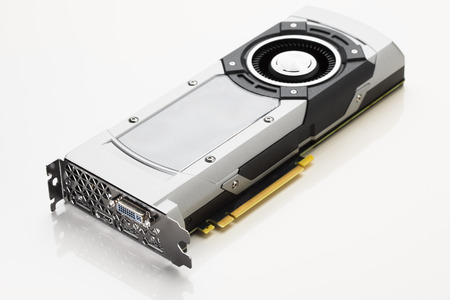
\includegraphics[width=0.5\linewidth]{fig/gpu.jpg}
\end{center}
\begin{center}
{\large Marc Fuentes - INRIA Pau\\ }
\end{center}
\end{frame}

%****************************************************************
% Xedea
%**************************************************************
\begin{frame}{Plan}
\begin{itemize}[<+->]
   \item Découverte
     \begin{itemize}
       \item Exemple d'applications 
       \item Prolégomènes (parallèlisme, mémoire, cache)
       \item Exemple d'introduction
       \item Modèle d'exécution d'un GPU
       \item Accès mémoires et coalescence
       \item Outils (déverminage, profilage)
     \end{itemize}
 \item Optimisation 
     \begin{itemize}
       \item Facteurs limitants (mémoire, instructions, latence)
       \item Métriques (BP, occupation)
       \item Transferts hôte \geziBikoitz\ accélérateur
       \item Mémoires de l'accélérateur
       \item Divergence de threads \& réductions
     \end{itemize}
  \item Divers
     \begin{itemize}
       \item Une brève histoire des GPUs
       \item Interfaces de programmation applicatives (IPA)
     \end{itemize}
\end{itemize}
\end{frame}

%****************************************************************
% lehen kapitulua
%****************************************************************
\begin{frame}
  \begin{center}
    {\Huge Première partie : Découverte}
  \end{center}
\end{frame}

%****************************************************************
% erabilpenak
%**************************************************************
\begin{frame}{Utilisation des GPU}
\pause
  \begin{itemize}[<+->]
    \item[\adibi]
      \begin{minipage}[c]{0.49\linewidth}
        calcul haute performance (HPC) : simulation numérique de grande taille
      \end{minipage}
      \begin{minipage}[c]{0.49\linewidth}
        \begin{figure}
        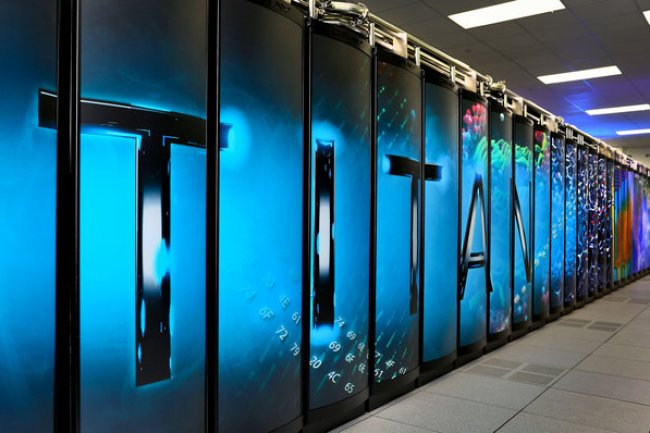
\includegraphics[width=0.6\linewidth]{fig/titan.jpg}
          \caption{\tiny Supercalculateur Titan : $\thicksim$ 18000 GPU}
        \end{figure}
      \end{minipage}
    \item[\adibi]  \begin{minipage}[l]{0.49\linewidth}
     traitement d'image, jeux vidéos 
      \end{minipage}
      \begin{minipage}[r]{0.49\linewidth}
        \begin{figure}
        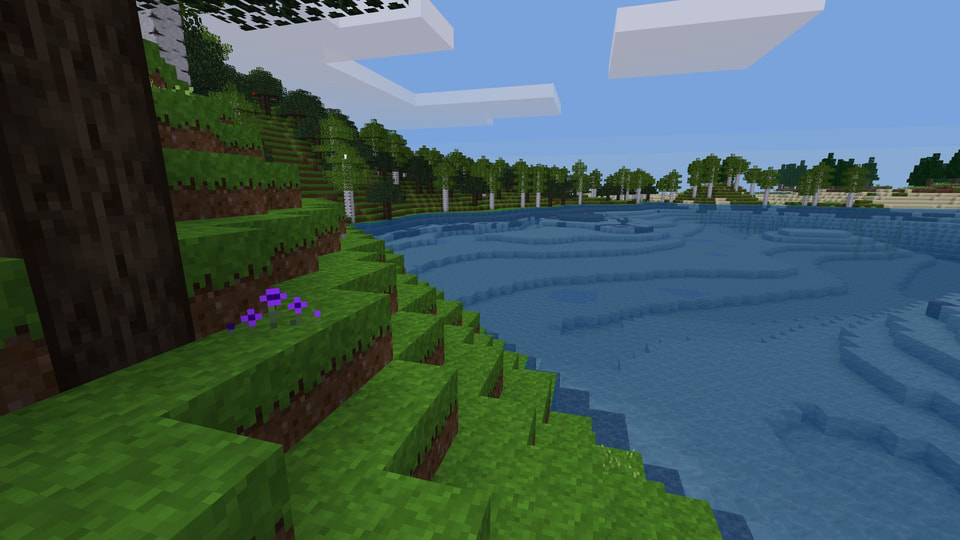
\includegraphics[width=0.6\linewidth]{fig/minetest.jpg}
          \caption{\tiny Minetest (clone libre) }
        \end{figure}
      \end{minipage}
    \item[\adibi]  \begin{minipage}[l]{0.49\linewidth}
     apprentissage automatique
      \end{minipage}
      \begin{minipage}[r]{0.49\linewidth}
        \begin{figure}
        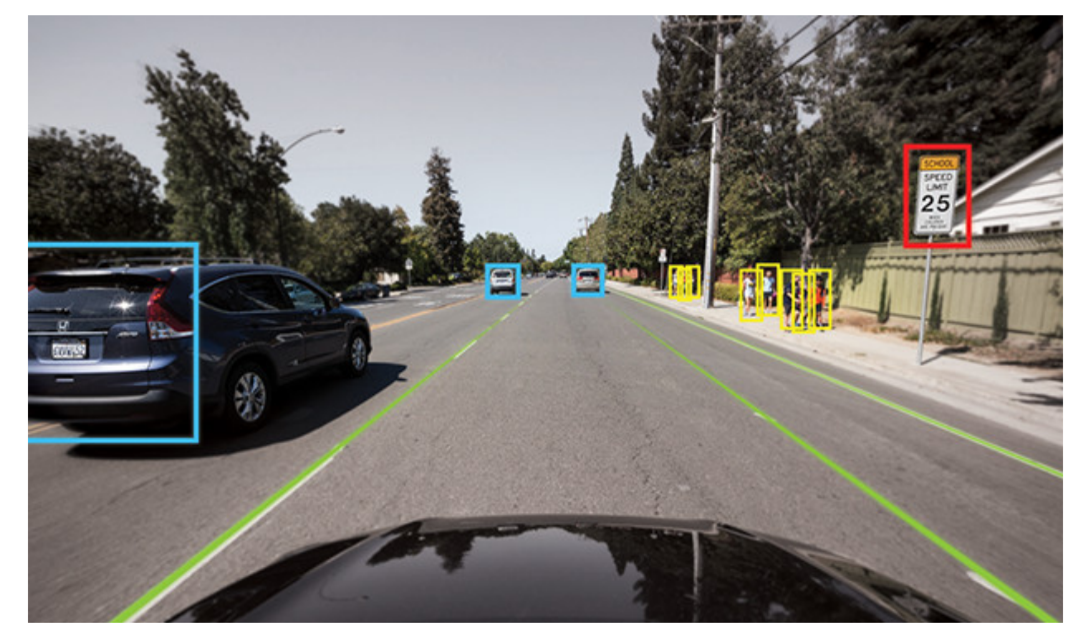
\includegraphics[width=0.6\linewidth]{fig/neural.png}
          \caption{\tiny véhicule autonome(projet inutile \faMehO)}
        \end{figure}
      \end{minipage}
  \end{itemize}
\end{frame}

%****************************************************************
% Paralelismo : partekatu edo banatu
%****************************************************************
\begin{frame}{Parallèlisme}{partagé/distribué}
\pause
La mémoire utilisée peut être distribuée ou partagée.
  \begin{itemize}[<+->]
    \item mémoire partagée : on a des threads (fils d'exécution) ou tâches qui accèdent à une mémoire commune. 
      \begin{itemize}
        \item[\pozik] rapidité d'accés en lecture/écriture
        \item[\kontuz] accés concurrents : utilisation de verrous ou d'opérations atomiques
        \item[\argi] cibles : Threads Posix, OpenMP, CUDA
      \end{itemize}
    \item mémoire distribuée : chaque processus a une mémoire privée et communique avec les autres par des messages
      \begin{itemize}
        \item[\argi] nécéssaire sur de très grands problèmes (limite mémoire/nœud moins gênante)
        \item[\triste] envoie de messages peut être couteux
        \item[\argi] cibles : MPI, Multi-GPU
      \end{itemize}
  \end{itemize}
\end{frame}

%****************************************************************
% Paralelismoa : alea
%****************************************************************
\begin{frame}{Parallèlisme}{Grain}
\begin{itemize}[<+->]
  \item[\faTruck] gros grain : un processeur parallèle (tâche, threads, processus MPI) traite beaucoup d'éléments 
   \begin{itemize}
     \item décomposition de domaine (maillage, matrice) :  ex. MUMPS
     \item parallèlisme par tâches (ex : STARPU)
     \item[\hand] chaque processeur doit avoir suffisament de mémoire pour traiter une grosse tâche
     \item[\argi] nombre raisonnable de tâches
   \end{itemize}
 \item[\faBicycle] grain fin : chaque processeur traite une «donnée élémentaire»
   \begin{itemize}
     \item[\hand] nécessite un grand nombre de threads
     \item[\hand] le changement de contexte doit être négligeable
     \item[\argi] trés grand nombre de tâches $\geqslant 10000$
   \end{itemize}
\end{itemize}
\end{frame}

%****************************************************************
% Paralelismoa : arkitektura
%****************************************************************
\begin{frame}{Parallèlisme}{Architecture}
\begin{itemize}[<+->]
  \item homogène : caractéristiques semblables(latence, mémoire, etc)
   \begin{itemize}
     \item processeurs vectoriels (Cray, DEC)
     \item modèle SIMD : MMX, SSE, AVX, Altivec
     \item grappe de calcul MPI avec des nœuds identiques
   \end{itemize}
  \item hétérogène : disparités entre les processeurs
   \begin{itemize}
     \item Calcul sur GPU : hôte vs accélérateur
     \item \begin{minipage}[r]{0.49\linewidth} 
         Processeur Cell dans les PS3 
      \end{minipage}
      \begin{minipage}[r]{0.49\linewidth}
        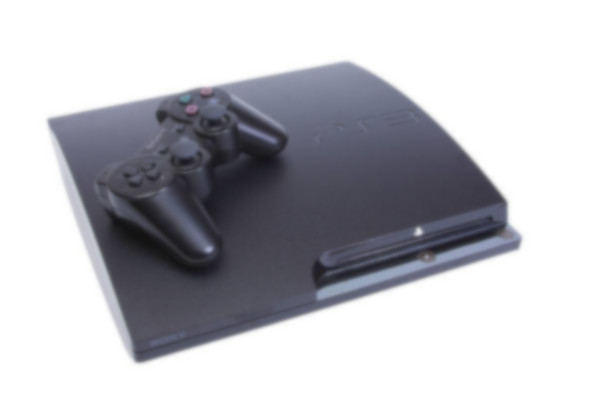
\includegraphics[width=0.6\linewidth]{fig/ps3_lauso.jpg}
      \end{minipage}
\end{itemize}
\end{itemize}
\pause
  \hand\  La programmation sur GPU est {\it grosso modo}\  donc un parallèlisme à {\bf grain fin}, à mémoire {\bf partagée} tournant sur
  une architecture {\bf hétérogène}.
\end{frame}

%****************************************************************
% sarrera : memoria eta cachea (eskema)
%****************************************************************
\begin{frame}{Mémoire et Cache}{schéma}
\begin{itemize}[<+->]
  \item La rapidité d'exécution d'un calcul dépend aussi de la «proximité» avec le CPU de l'élément de mémoire à traiter 
  \item[\gezi] les concepteurs de CPU ont créé des {\bf caches} pour stocker les valeurs mémoires les plus utilisées
  \begin{center}
    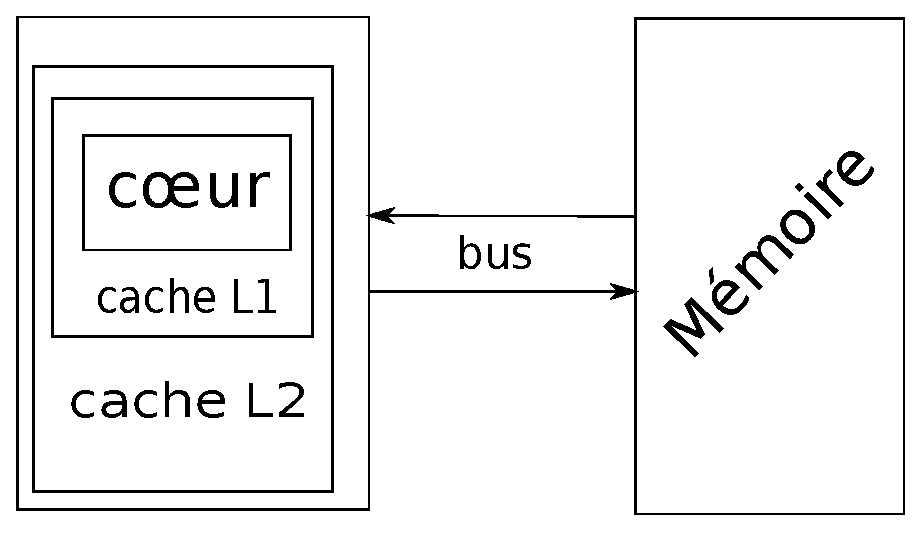
\includegraphics[width=0.7\linewidth]{fig/cpu_classique.eps}
  \end{center}
\end{itemize}
\end{frame}

%****************************************************************
% sarrera : latentzia
%****************************************************************
\begin{frame}{Mémoire et Cache (II)}{latence}
\pause
  \begin{itemize}[<+->]
  \item ainsi la latence $l$ de l'emplacement mémoire auquel on accède  respecte
  $$l({\mbox{\scriptsize registre}}) \leqslant l(\mbox{\scriptsize cache L1}) \leqslant
    l(\mbox{\scriptsize cache L2}) \leqslant l(\mbox{\scriptsize mémoire globale}).$$
  \item ordres de grandeur des latences (core i7 Xeon E5500)
    \begin{tabular}{|l|c|c|}
    \hline
      type & nb cycles & latence (ns)  \\
    \hline
      cache L1  &  4 & 2 \\
      cache L2  &  10 & 5 \\
      cache L3 (non partagé) & 40 & 20  \\
      cache L3 (partagé) &  65 & 35  \\
      mémoire vive locale & & 60 \\
      mémoire vive distante & & 100 \\
    \hline
    \end{tabular}
  \end{itemize}
\end{frame}

%%****************************************************************
%% sarrera : arrakasta ta huts
%%****************************************************************
\begin{frame}{Cache}{Succès et défauts}
\begin{itemize}[<+->]
  \item[\pozik] succès (hit) : accès déjà dans la ligne de cache 
  \item[\triste] défaut (miss) : accès hors de la ligne de cache \gezi\ il faut recharger entièrement la ligne de cache!
  \item[\argi] un code localisant ses accès dans le cache minimise les défauts de cache et tourne plus vite
  \item[\adibi] double boucle en C sur les lignes (resp. colonnes en Fortran)
\begin{minipage}[c]{0.49\linewidth}
  \lstinputlisting[language=C]{code/loop_col.c}
\end{minipage}
\begin{minipage}[r]{0.49\linewidth}
    \begin{tabular}{|c|c|}
    \hline
     boucle ext. & tps(s)  \\
    \hline
      i (lignes) & 2.7s \\
      j (cols)  & 3.4s \\
    \hline
    \end{tabular}
\end{minipage}
\item[\hand] raison d'être des biblios BLAS et LAPACK
\end{itemize}
\end{frame}

%%****************************************************************
%% sarrera : 
%%****************************************************************
%%%\begin{frame}{Passage à l'échelle}
%%%\begin{itemize}[<+->]
%%%  \item fort (strong scalability)
%%%    \begin{itemize} 
%%%       \item loi d'Amdhal (pessimiste)
%%%    \end{itemize}
%%%  \item faible (weak scalability)
%%%    \begin{itemize}
%%%      \item loi
%%%    \end{itemize}
%%%\end{itemize}
%%%\end{frame}

%%****************************************************************
%% Exemple introductif (séquentielle)
%%****************************************************************
\begin{frame}{Exemple d'introduction}{version séquentielle}
\pause
\begin{itemize}[<+->]
  \item[\adibi] soit un programme calculant \texttt{tab[:]} $\leftarrow$ \texttt{tab[:] + 3}
\lstinputlisting{code/increment.c}
\item[\galde] on souhaite paralléliser la boucle en ligne 6 à l'aide de CUDA
\end{itemize}
\end{frame}

%%****************************************************************
%% Exemple introductif (CUDA)
%%****************************************************************
\begin{frame}{Exemple d'introduction}{version CUDA}
\pause
\begin{itemize}[<+->]
  \item[\adibi] on peut écrire le programme suivant
\lstinputlisting{code/incrementGPU.cu}
\item[\pozik] plus de boucle
\item[\argi] nouveaux mot-clefs : \texttt{\_\_global\_\_, threadIdx}
\item[\argi] appel du noyau \texttt{increment<<<1,N>>>}
\item[\argi] gestion de la mémoire : \texttt{\small cudaMemcpy, cudaMalloc, cudaFree}
\end{itemize}
\end{frame}

%****************************************************************
% Exemple introductif principe
%****************************************************************
\begin{frame}{Exemple d'introduction}{explication}
\pause
\begin{itemize}[<+->]
 \item[\argi] boucle \texttt{for} \gezi\ appel d'un {\bf thread}
 \item[\argi] exécutant le noyau \texttt{increment}
 \item[\argi] pour chaque indice de boucle indexé par \texttt{threadIdx.x}
 \item[\argi] sur le tableau \texttt{tab\_d} alloué sur le GPU
 \item[\kontuz] il faut copier \texttt{tab} sur le GPU et le rapatrier après calcul
\end{itemize}
\pause
\begin{center}
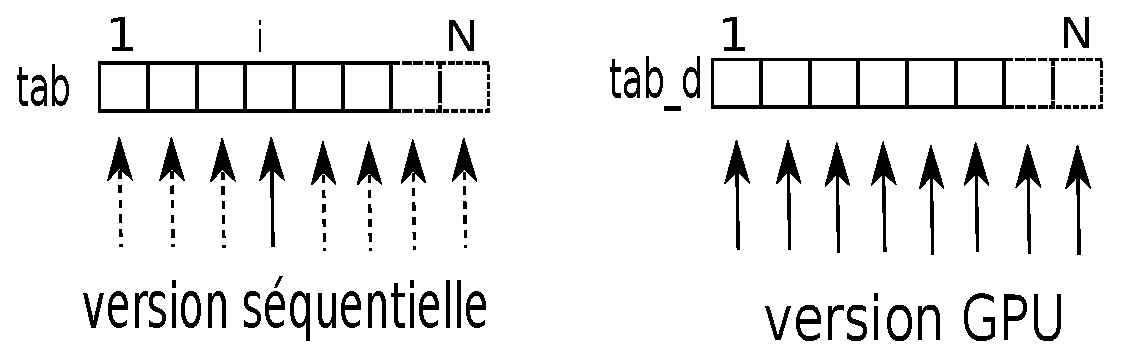
\includegraphics[width=0.9\linewidth]{fig/parallel.eps}
\end{center}
\end{frame}

%****************************************************************
% Déroulé classique d'un calcul
%****************************************************************
\begin{frame}{Déroulé typique d'un calcul}
  \lstset{basicstyle=\ttfamily}
\pause
  \begin{itemize}[<+->]
    \item[\argi] un programme CUDA suit généralement les étapes suivantes 
\begin{enumerate}[<+->]
 \item allouer la mémoire sur le GPU : \lstinline!cudaMalloc!
 \item copier depuis la mémoire globale vers le GPU : \lstinline!cudaMemCpy( ... ,cudaMemcpyHostToDevice)!
 \item exécuter le noyau sur l'accélerateur : \lstinline!myKernel<<<...,...>>>(...)!
 \item rapatrier les résultats en mémoire globale \lstinline!cudaMemCpy(...,cudaMemcpyDeviceToHost)!
 \item libérer la mémoire sur le GPU \lstinline!cudaFree!
 \item visualiser les résultats
\end{enumerate}
\item[\geldi] Avant de poursuivre, nous avons besoin de comprendre le modèle d'exécution sur GPU
\end{itemize}
\end{frame}

%****************************************************************
% Modèle d'execution GPU I
%****************************************************************
\begin{frame}{Modèle d'exécution du GPU}{exemple sur un Tesla C1060}
\begin{minipage}[c]{0.49\linewidth}
\begin{itemize}
  \item multiprocesseur de flux (SM)
    \begin{itemize}
      \item groupe de 8 processeurs de flux (SP)
        \begin{itemize}
          \item partage de mémoire locale
          \item synchronisation
        \end{itemize}
    \end{itemize}
  \item processeur de flux (SP) : 
    \begin{itemize}
    \item 64KB de registres, 
    \item {\bf threads} : ensemble de registres
    \begin{itemize}
      \item création/destruction gratuites
    \end{itemize}
  \item exécution entrelacée de {\em threads} matériels : jusqu'à 128 par SP
    \end{itemize}
\end{itemize}
\end{minipage}
\begin{minipage}[c]{0.49\linewidth}
\begin{center}
  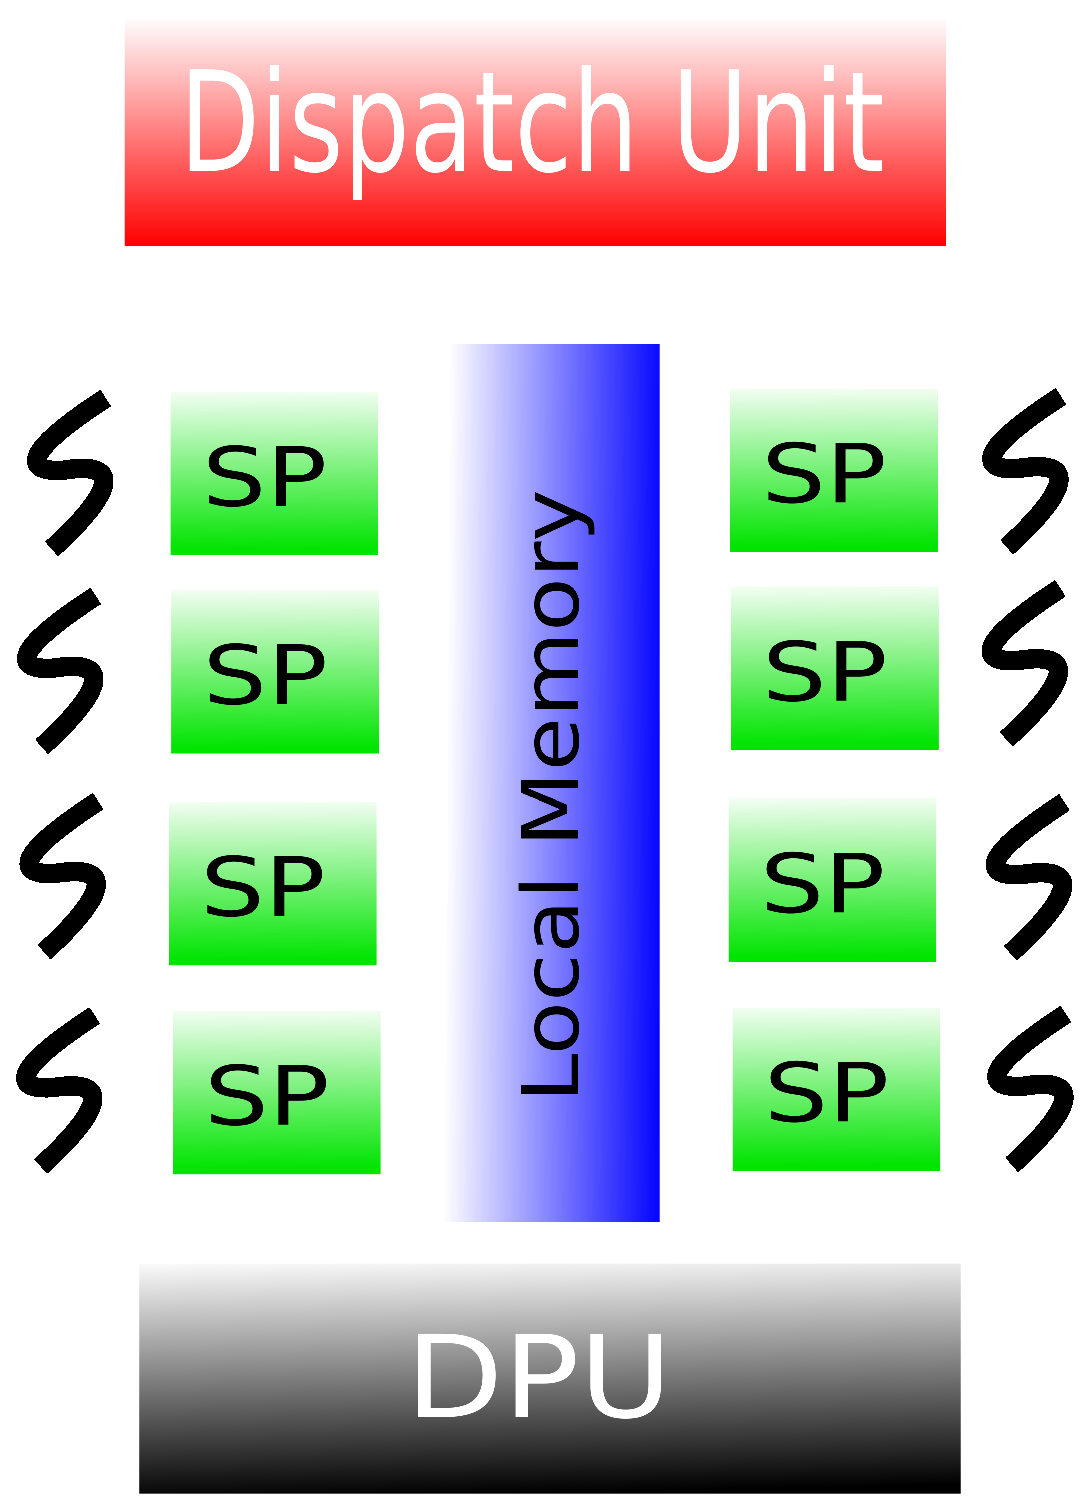
\includegraphics[width=0.6\linewidth]{fig/GPUArchiThread.eps}
\end{center}
\end{minipage}
\end{frame}

%****************************************************************
% Modèle d'execution GPU II
%****************************************************************
\begin{frame}{Modèle d'exécution du GPU}{exemple sur un Tesla C1060 (II)}
\begin{minipage}[c]{0.49\linewidth}
\begin{itemize}
  \item 1 seule unité d'envoi d'instruction par multiprocesseur de flux
    \begin{itemize}
      \item tous les SPs exécutent la même instruction au même cycle d'horloge
        \begin{itemize}
          \item sur des données différentes (SIMD)
        \end{itemize}
    \end{itemize}
  \item l'unité d'envoi prend 4 cycles pour récupérer et décoder les instructions
    \begin{itemize}
      \item 4 groupes de 8 {\bf threads} planifiés / ligne
    exécutant la même instruction
      \item changement de contexte gratuit !
    \end{itemize}
\end{itemize}
\end{minipage}
\begin{minipage}[c]{0.49\linewidth}
\begin{center}
  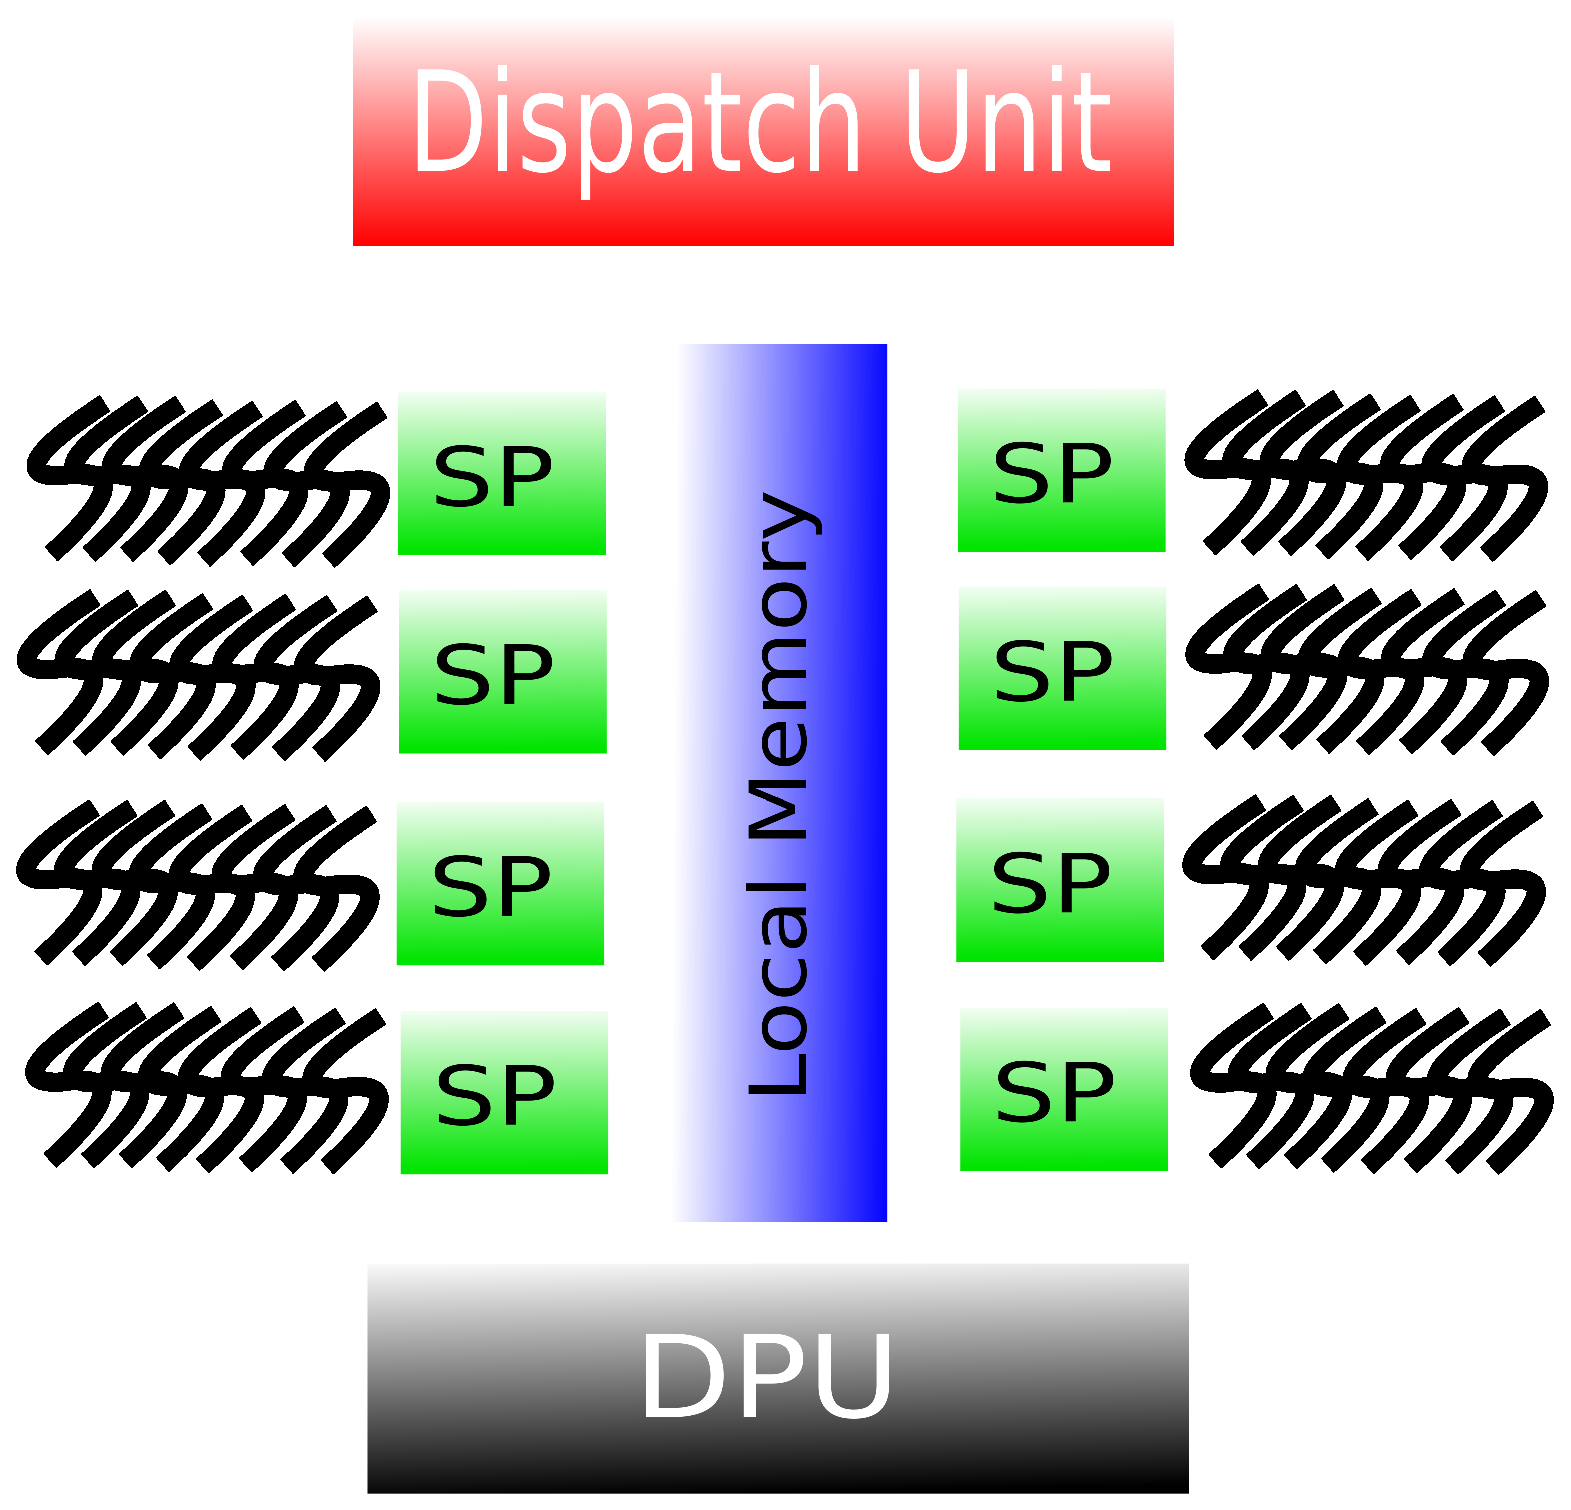
\includegraphics[width=0.9\linewidth]{fig/GPUArchi8Thread.eps}
\end{center}
\end{minipage}
\end{frame}

%****************************************************************
% Modèle d'execution GPU III
%****************************************************************
\begin{frame}{modèle d'exécution du GPU}{warps et demi-warps}
\begin{minipage}[c]{0.59\linewidth}
\begin{itemize}
  \item les {\bf threads} sont implicitement groupés en {\bf warps}
    \begin{itemize}
      \item un {\bf warp} (chaîne) = 32 threads 
      \item tous les threads d'une même chaîne exécutent la même instruction au même cycle logique
        \begin{itemize}
          \item[\kontuz] \alert{pas de divergence!}
        \end{itemize}
    \end{itemize}
  \item charger des données depuis la mémoire globale est coûteux
    \begin{itemize}
      \item plus de 4 threads nécessaires / SP
      \item 128 permettent de recouvrir la latence mémoire
    \end{itemize}
\end{itemize}
\end{minipage}
\begin{minipage}[c]{0.39\linewidth}
\begin{center}
  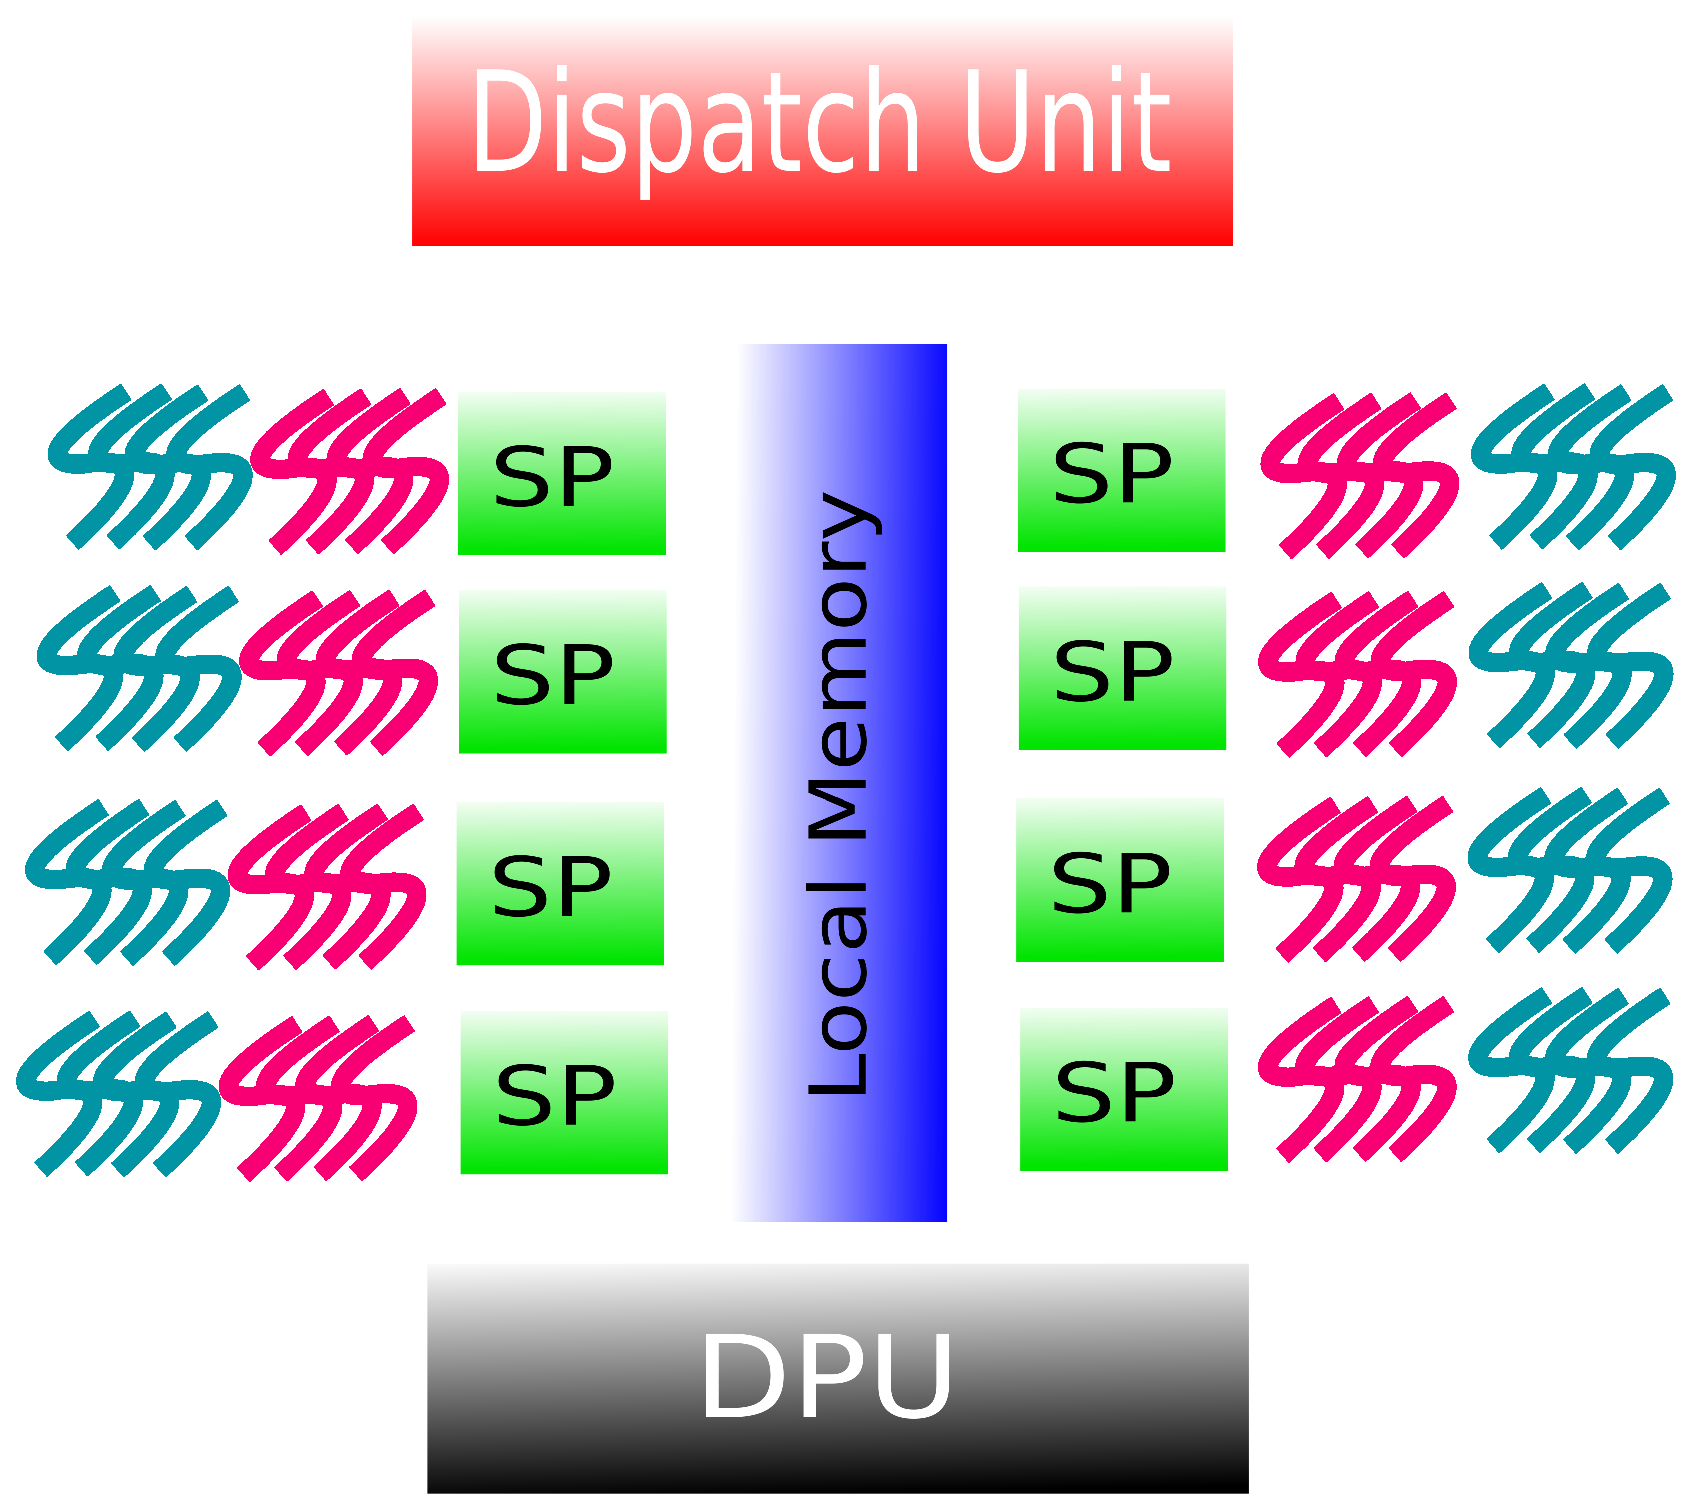
\includegraphics[width=0.95\linewidth]{fig/GPUArchi8ThreadDiv.eps}
\end{center}
\end{minipage}
\end{frame}

%****************************************************************
% Modèle d'execution GPU IV
%****************************************************************
\begin{frame}{modèle d'exécution du GPU}{exemple avec un K40M}
\begin{minipage}[c]{0.59\linewidth}
  \begin{itemize}[<+->]
    \item GPU = ensemble de multiprocesseurs de flux (SM) partageant une mémoire globale (DRAM)
    \item Tesla K40M : 
      \begin{itemize}
        \item 15 SM, 192 SP / SM $\Rightarrow$ 2880 SP
        \item 2048 threads max / SM $\Rightarrow$ 30.720 threads
      \end{itemize}
    \item threads «spéciaux»
      \begin{itemize}
        \item parallélisme de données respectant des motifs d'accès réguliers
      \end{itemize}
  \end{itemize}
\end{minipage}
\begin{minipage}[c]{0.39\linewidth}
\begin{center}
  \rotatebox{90}{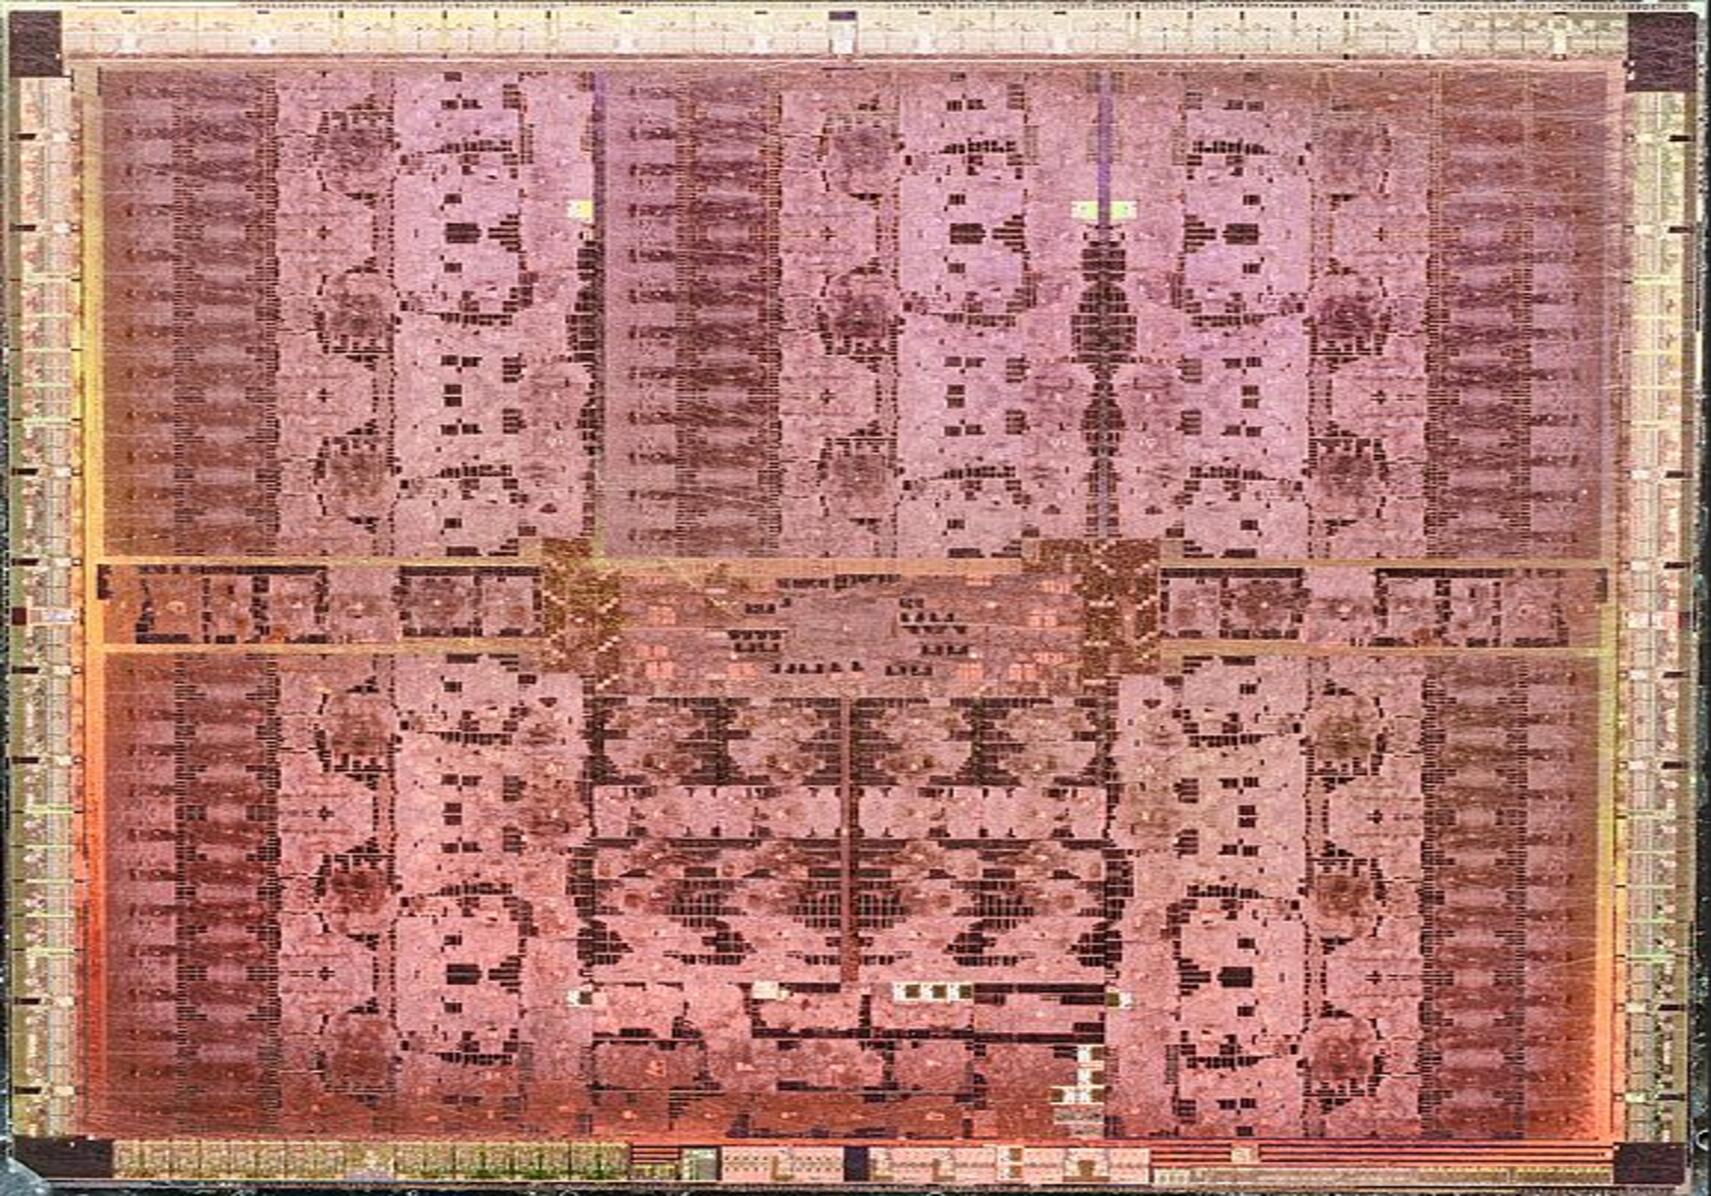
\includegraphics[width=0.9\linewidth]{fig/kepler.jpg}}
\end{center}
\end{minipage}
\end{frame}

%****************************************************************
% Organisation des threads
%****************************************************************
\begin{frame}{Organisation des threads}{découpage des données}
 \pause
 \begin{minipage}[c]{0.59\linewidth}
  \begin{itemize}[<+->]
    \item[\argi] K40M $\approx$ 30K threads 
    \item[\galde] Que faire si $N \geq 30K$ ?
    \item[\scout] on découpe les données en blocs
    \item[\argi] threads organisés en {\em blocs} qui tournent chacun sur 1 SM
    \item[\argi] une {\bf grille} répartie les blocs sur tous les SMs
    \item[\argi] on paramètre l'appel du noyau \texttt{myKernel<<<dg,db>>>} 
      \begin{itemize}
        \item dg : taille grille (\texttt{int} ou \texttt{dim3})
        \item db : taille bloc (\texttt{int} ou \texttt{dim3})
      \end{itemize}
  \end{itemize}
\end{minipage}
\begin{minipage}[c]{0.39\linewidth}
\begin{center}
  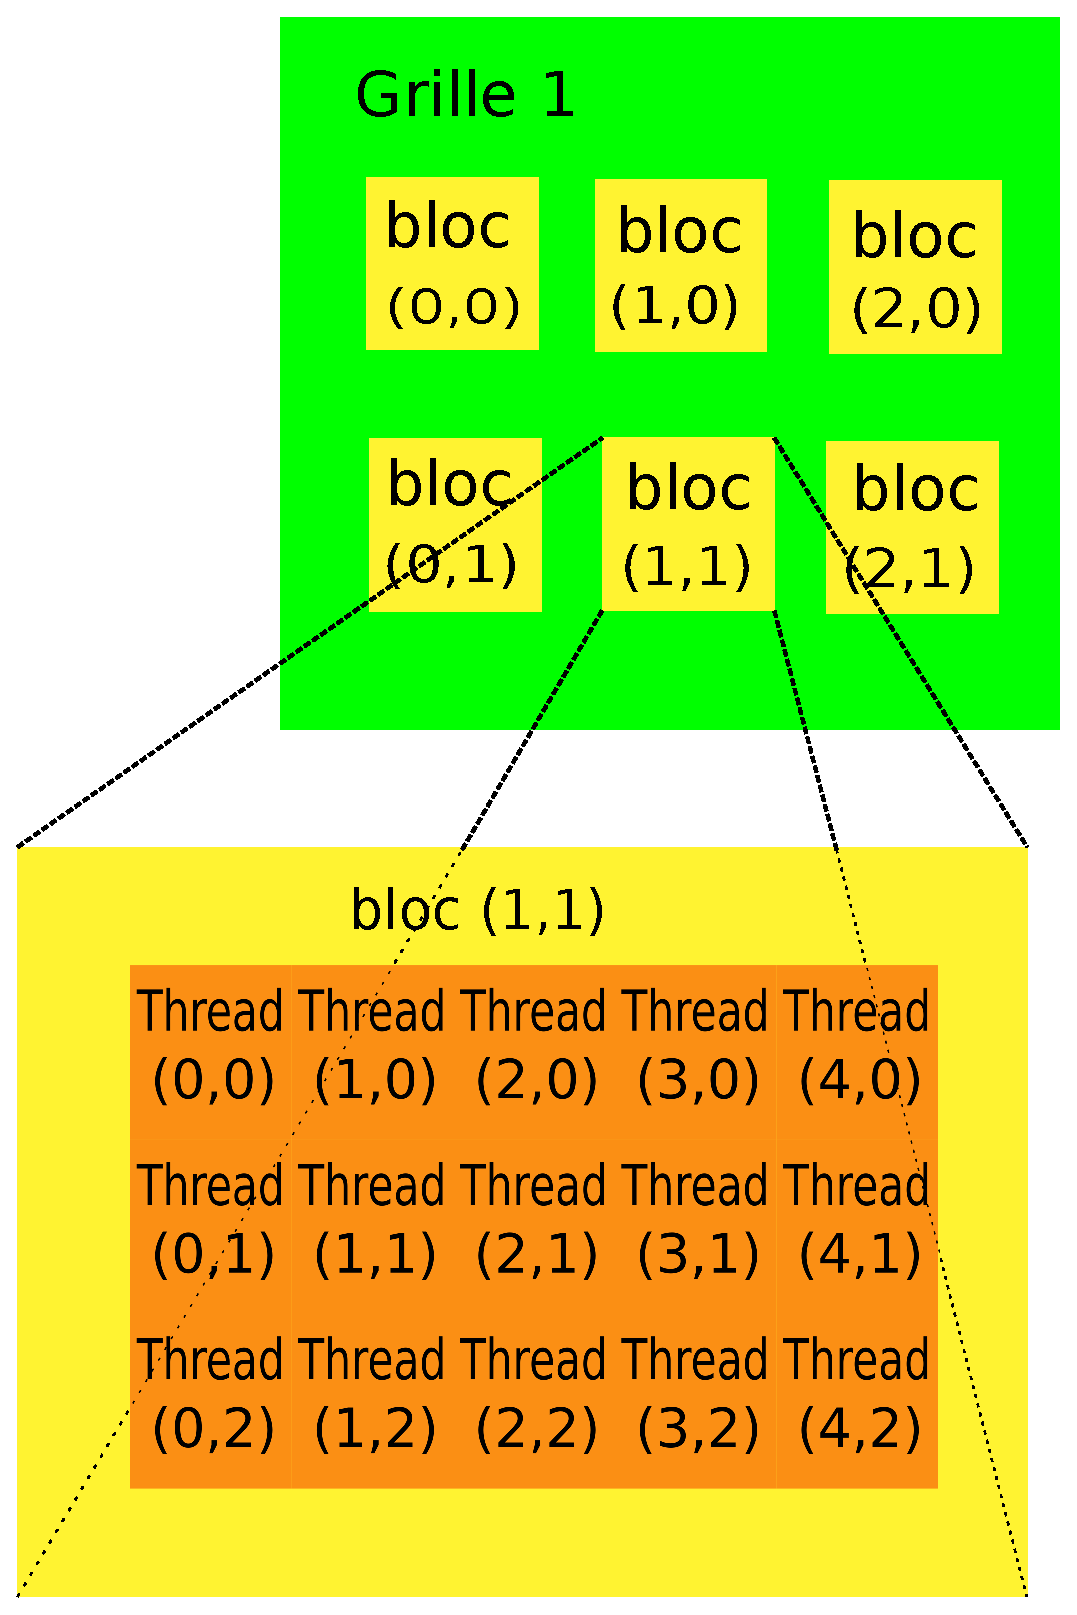
\includegraphics[width=0.8\linewidth]{fig/grille_et_blocs.eps}
\end{center}
\end{minipage}
\end{frame}

%****************************************************************
% Organisation des threads II
%****************************************************************
\begin{frame}{Organisation des threads}{ordonnancement}
 \pause
 \begin{minipage}[c]{0.59\linewidth}
   {\bf Le programme sur l'hôte demande l'exécution d'une grille de blocs de threads}
  \begin{itemize}[<+->]
    \item l'ordonnanceur de bloc distribue les blocs sur les SMs
    \item[\kontuz] des GPUs différents peuvent exécuter différemment la même grille de blocs
  \end{itemize}
\end{minipage}
\begin{minipage}[c]{0.39\linewidth}
\begin{center}
  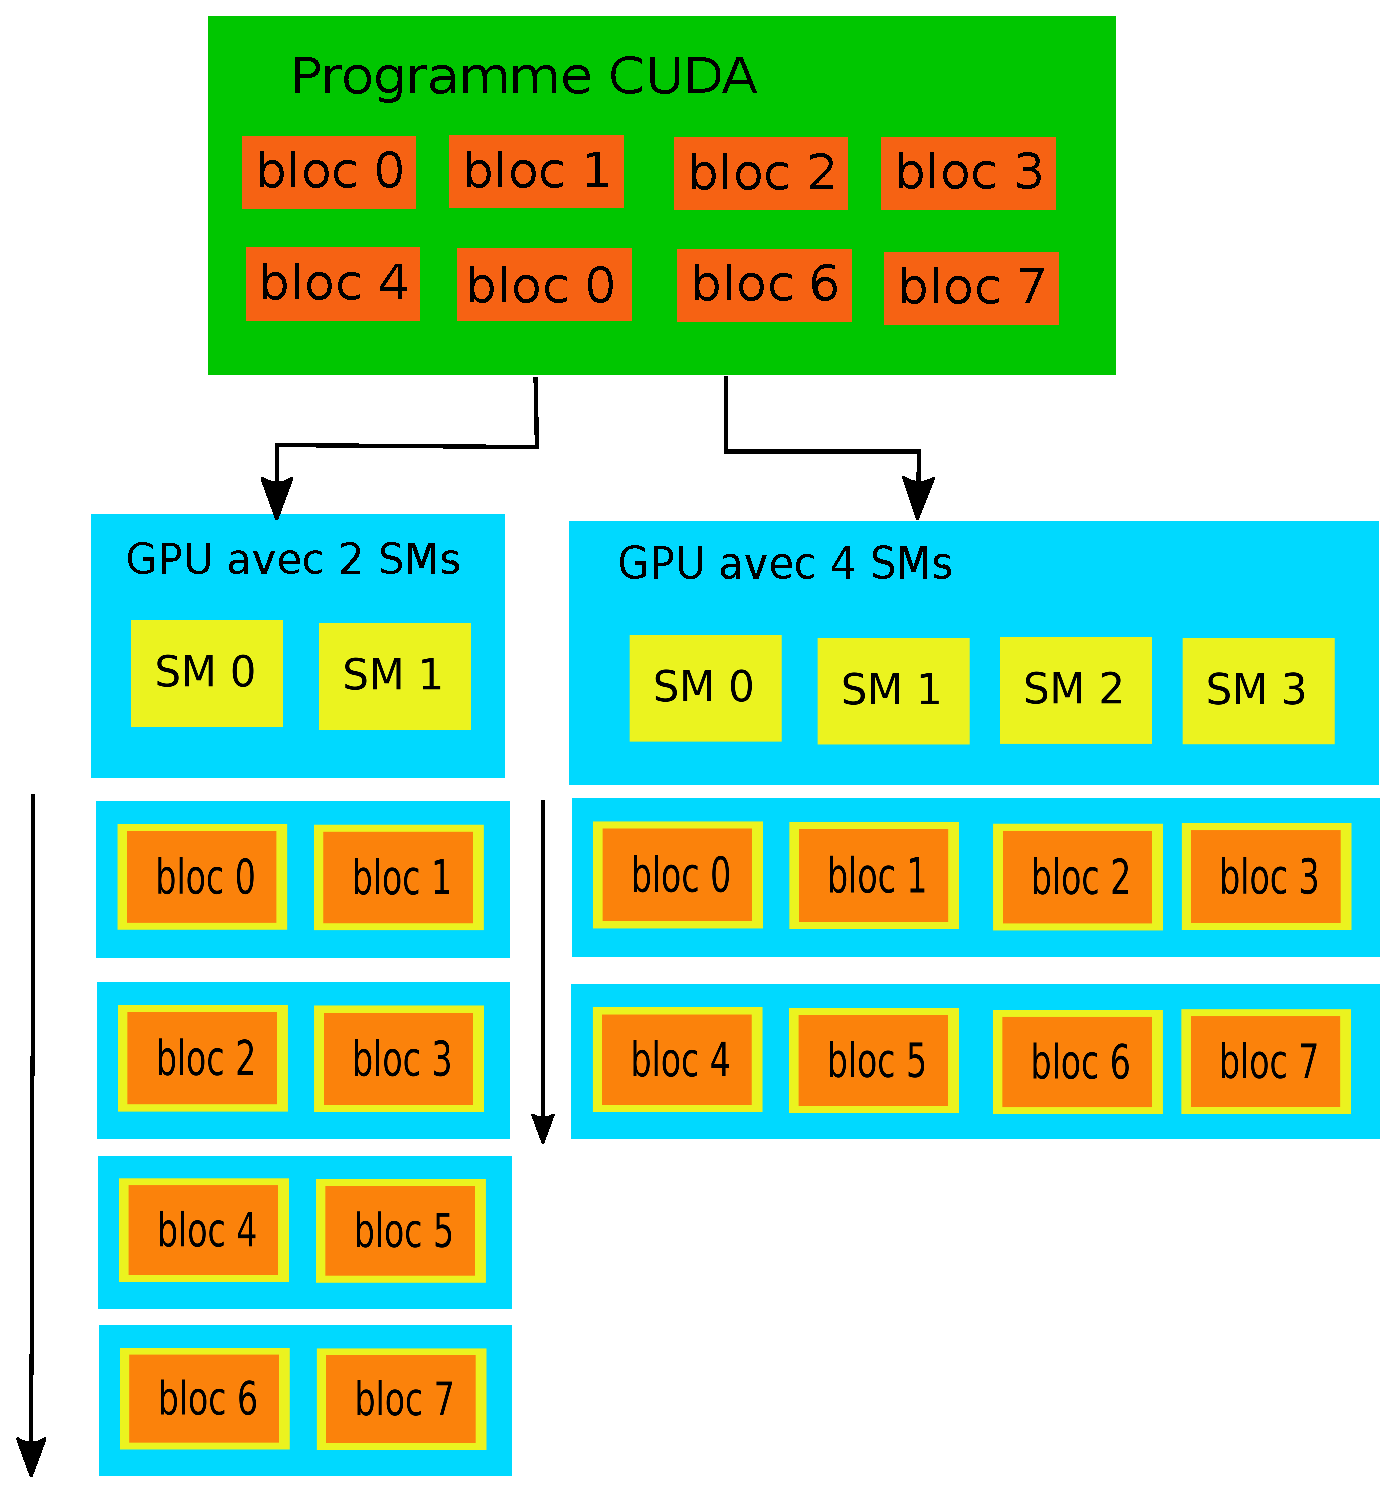
\includegraphics[width=0.95\linewidth]{fig/bloc_ordonanceur.eps}
\end{center}
\end{minipage}
\end{frame}

%****************************************************************
% Tailles des grilles/blocs 
%****************************************************************
\begin{frame}{Tailles de grille et de blocs}
  \begin{itemize}[<+->]
    \item[\argi] type CUDA pour gérer les dimensions de grille et de bloc
    \begin{itemize}
      \item \alert{dim3} est une structure avec 3 champs entiers \texttt{\_.x,\_.y et \_.z}
      \item soit \texttt{dg} un descripteur de grille et \texttt{db} un descripteur de bloc
    \end{itemize}
  \item[\argi] Limites de bloc 3D
   \begin{itemize}
     \item \texttt{db.x} $\leqslant 1024$, \texttt{db.y} $\leqslant 1024$, \texttt{db.z} $\leqslant 64$ 
     \item nb total de threads par bloc $\leqslant 1024$
     \item problèmes 2D \gezi\  \texttt{db.z} = 1 
     \item problèmes 1D \gezi\  \texttt{db.z} = \texttt{db.y} = 1
   \end{itemize}
 \item[\argi] limites de la grille 3D
   \begin{itemize}
     \item \texttt{dg.x} $\leqslant 2^{31}-1$, \texttt{dg.y} $\leqslant 2^{16} - 1 $, \texttt{dg.z} $\leqslant 2^{16}-1$
     \item nb total de threads par bloc $\leqslant 1024$
     \item problèmes 2D \gezi\  \texttt{dg.z} = 1 
     \item problèmes 1D \gezi\  \texttt{dg.z} = \texttt{dg.y} = 1
  \end{itemize}
\item[\adibi] exemple avec données 2D mais une grille 1D
  \lstinputlisting[language=C]{code/grille.c}
 \end{itemize}
\end{frame}

%****************************************************************
% Tailles des grilles/blocs
%****************************************************************
\begin{frame}{Taille de blocs}
  \begin{itemize}[<+->]
    \item[\scout] Pour des raisons d'alignement on choisit toujours des blocs de taille multiple de 32 (ou 16 pour les archi $\leqslant$ 1.x)
    \item[\galde] comment faire si les données ne sont pas multiples de la taille du bloc ?
    \item[\argi] on alloue en faisant un dépassement systématique et on fait une vérification dans le noyau
    \item exemple : pour une grille 1D
  \begin{itemize}
    \item[\egia] on choisit \texttt{GRID\_SIZE} = (N-1) / \texttt{BLOCK\_SIZE} + 1
\begin{center}
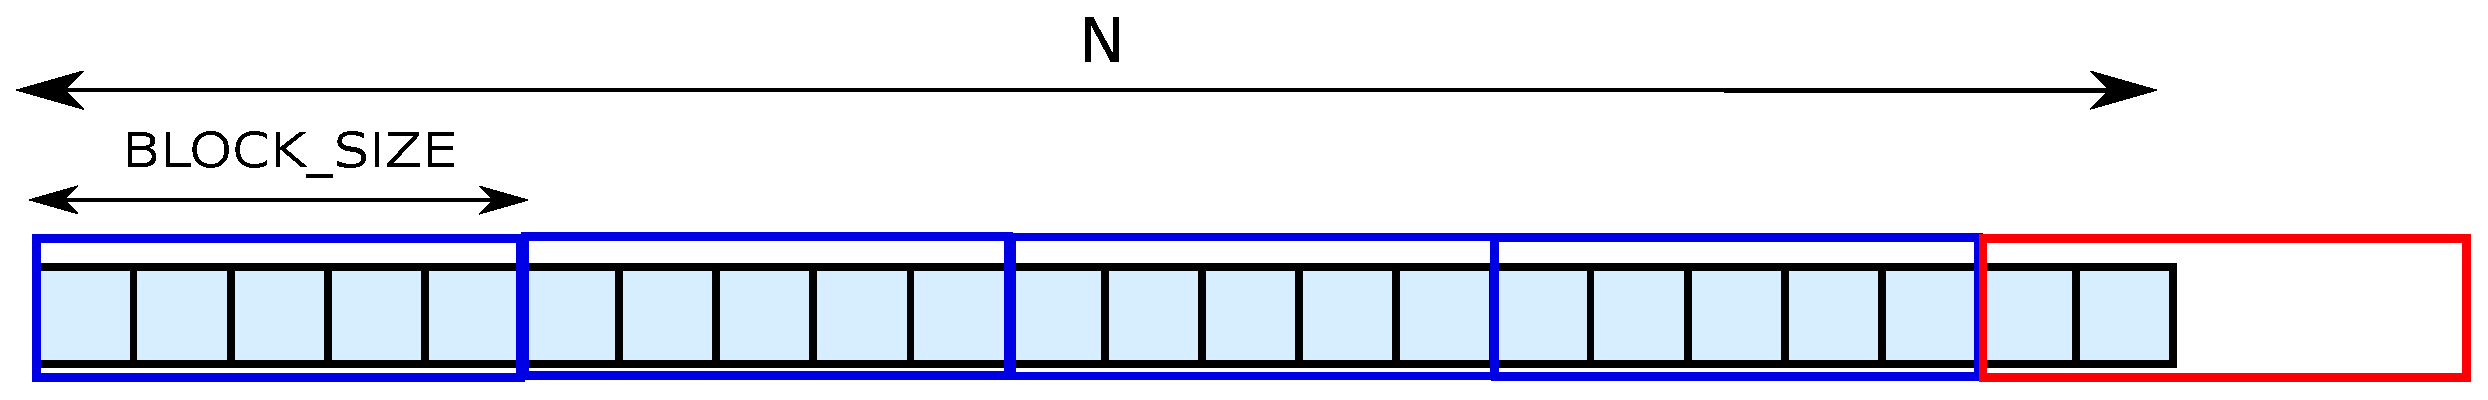
\includegraphics[width=0.7\linewidth]{fig/grille_1D.eps}
\end{center}
   \item[\egia] \texttt{\small currentIndex = blockDim.x * blockIdx.x + threadIdx.x}
   \item[\kontuz] penser à vérifier que \texttt{currentIndex} $\leq$ N !
 \end{itemize}
  \end{itemize}
\end{frame}

%****************************************************************
% Tailles des grilles/blocs
%****************************************************************
\begin{frame}{Taille de blocs}{Exemple XOR}
\begin{flushright}

\includegraphics[width=0.1\linewidth]{fig/xor.jpg}
\end{flushright}
  \lstinputlisting[language=C]{code/overflow.cu}
\end{frame}

%****************************************************************
% Coalescence
%****************************************************************
\begin{frame}{Coalescence}
  \begin{itemize}[<+->]
    \item[\argi] chaîne (warp) permet jusqu'à 32 accès mémoire concurrents
    \item[\argi] un accès mémoire typique $\thicksim$ 4 octets
    \item[\argi] granularité mémorielle : de 32 à 128 octets 
    \item[\harritu] {\em coalescence} : agrégation de plusieurs accès mémoire en un seul lorsqu'il se font dans le même bloc
    \item[\adibi] exemples avec 4 threads par chaîne et 4 mots par transaction
\begin{center}
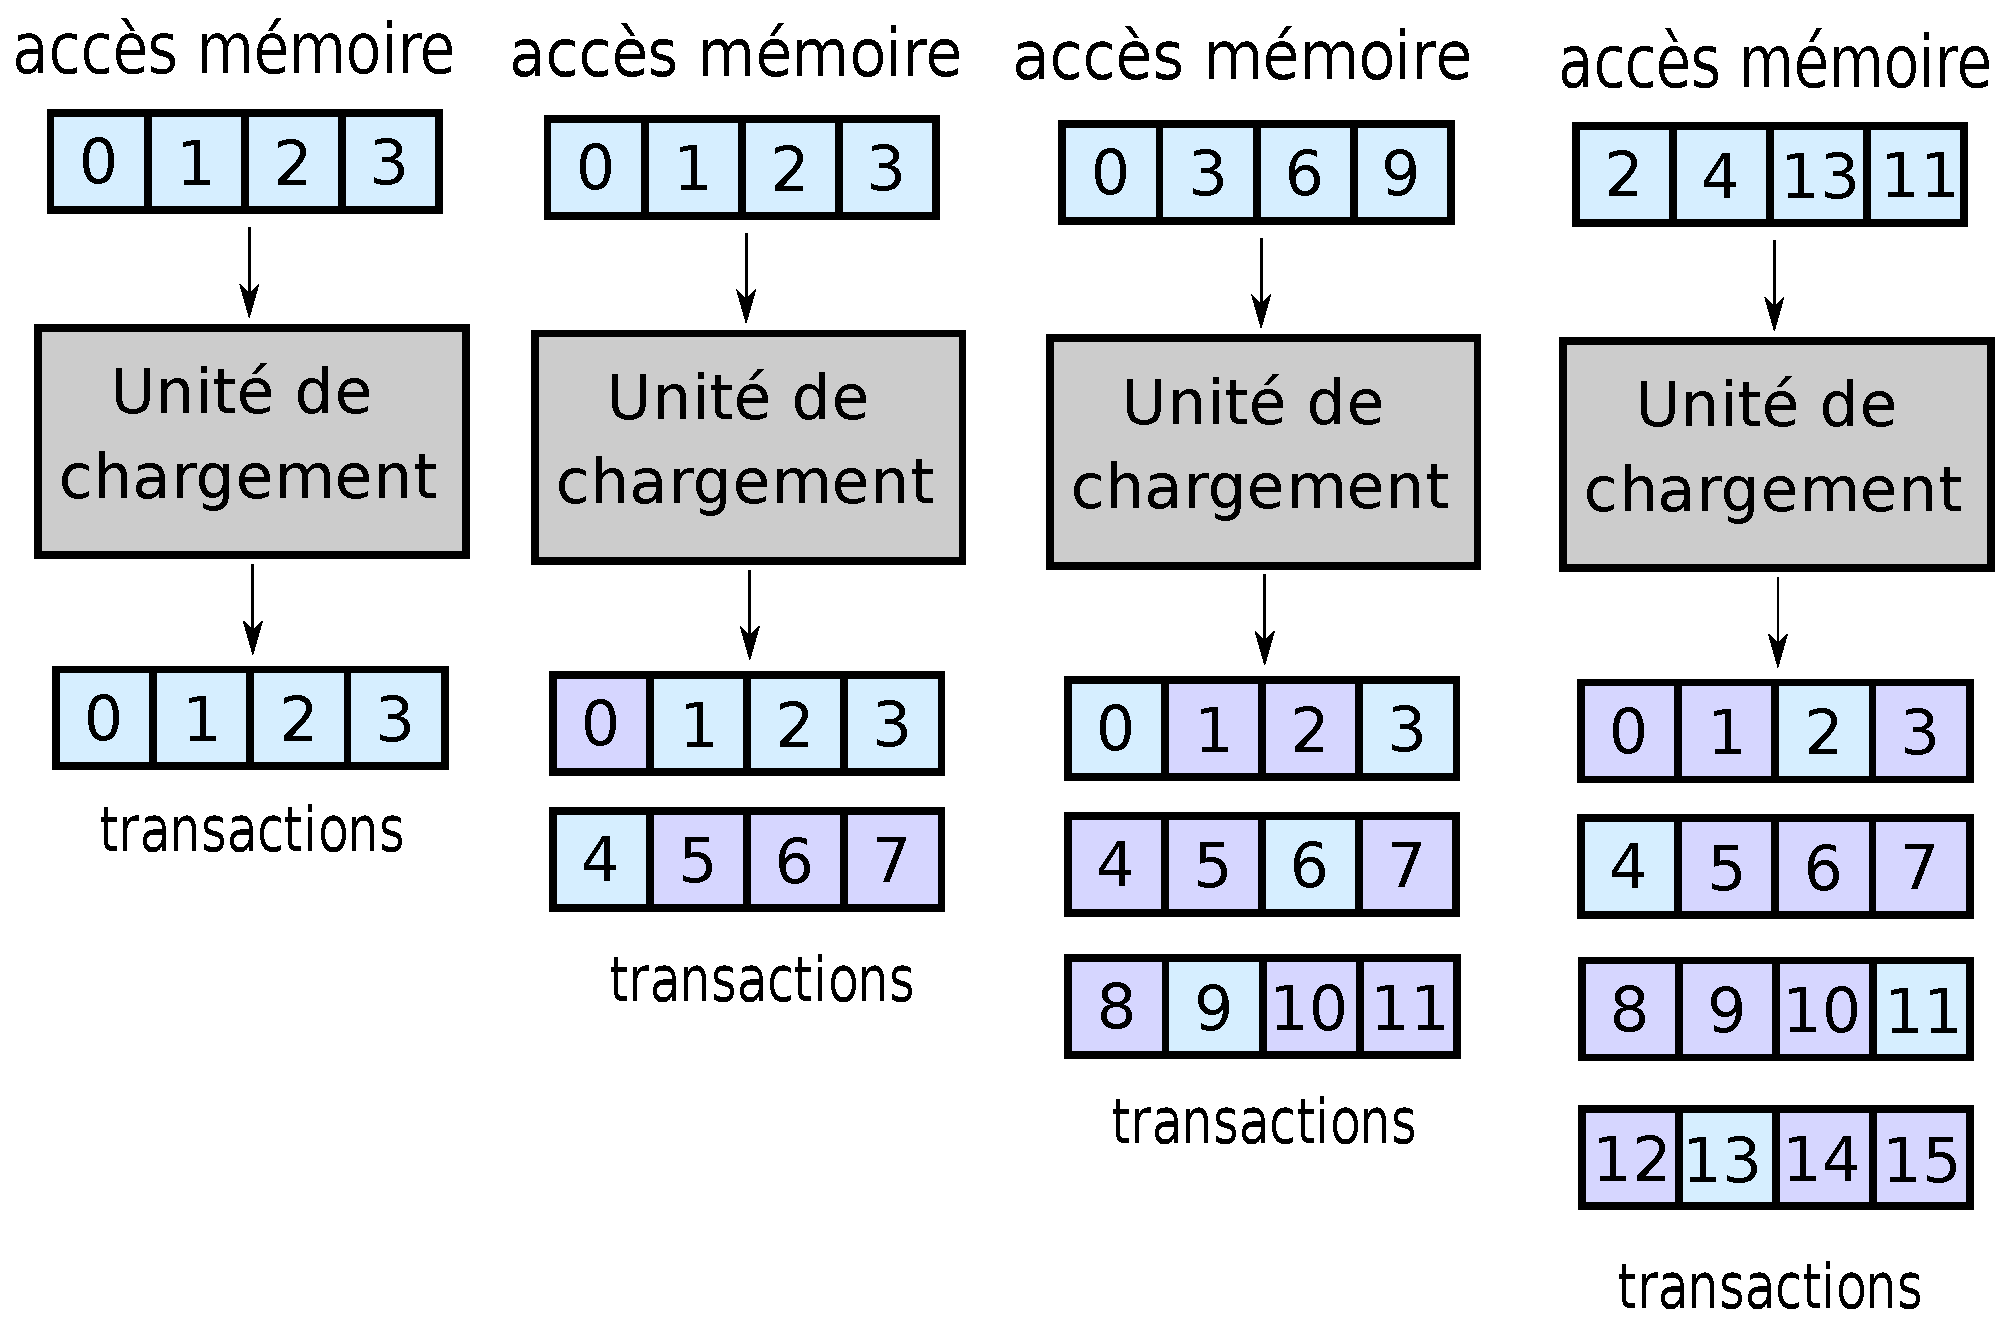
\includegraphics[width=0.6\linewidth]{fig/coalescence.eps}
\end{center}
  \end{itemize}
\end{frame}

%****************************************************************
% Coalescence
%****************************************************************
\begin{frame}{Coalescence}{Accès mémoires contigus}
  \begin{itemize}[<+->]
    \item[\adibi] soit le code d'homothétie d'un vecteur
\begin{center}
\lstinputlisting[language=C]{code/scale.c}
\end{center}
    \item[\argi] on a des accès {\em contigus}, ce qui autorise la coalescence
\begin{center}
  \vspace{0.5cm}
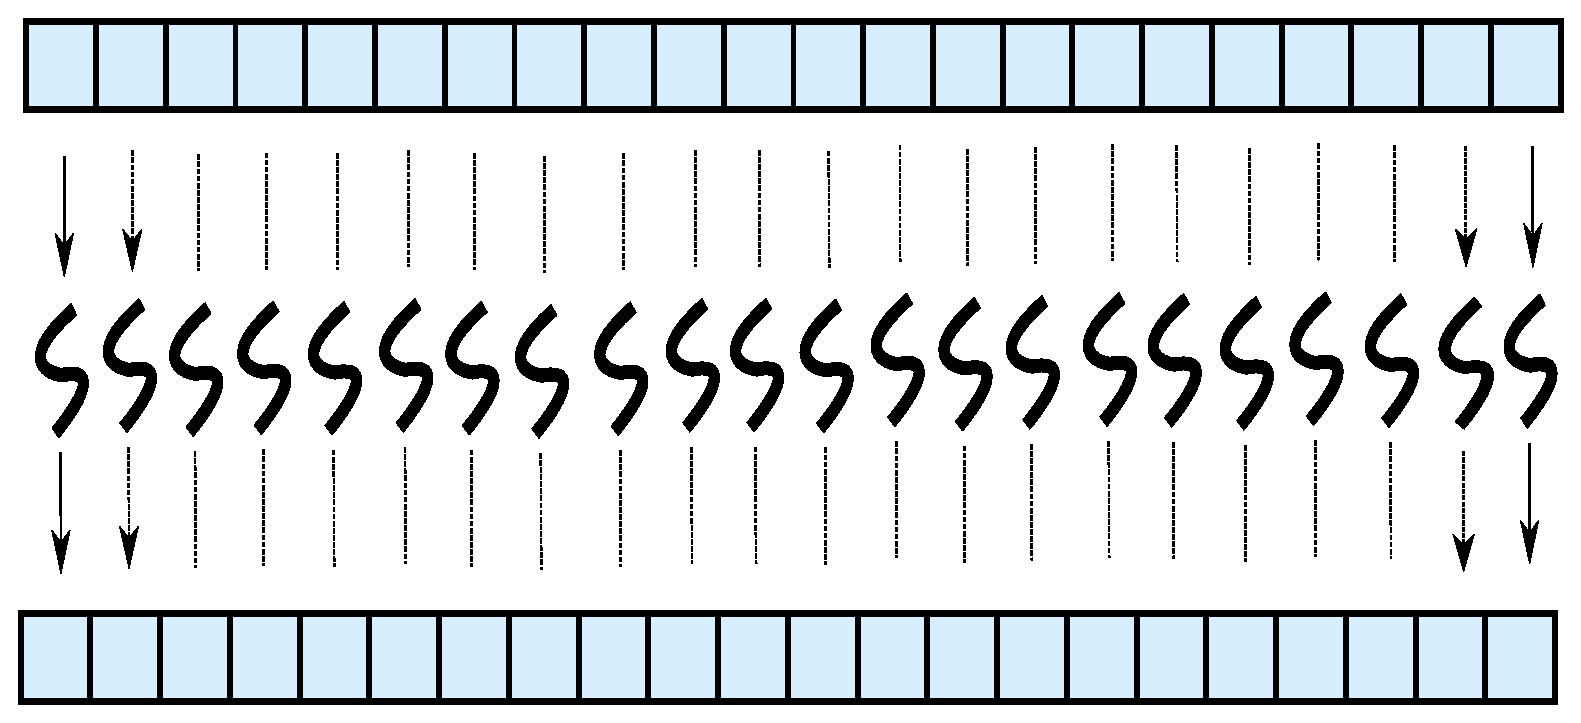
\includegraphics[width=0.8\linewidth]{fig/coalScale.eps}
\end{center}
  \end{itemize}
\end{frame}

%****************************************************************
% Coalescence
%****************************************************************
\begin{frame}{Coalescence}{Accès mémoires non contigus}
  \begin{itemize}[<+->]
    \item[\adibi] on peut y accéder différement, par exemple avec un pas de 2
\begin{center}
  \lstinputlisting[language=C]{code/scaleFlipAndHalf.c}
\end{center}
    \item[\kontuz] mais les tranferts mémoires sont non-coalescents !
\begin{minipage}[c]{0.49\linewidth}
  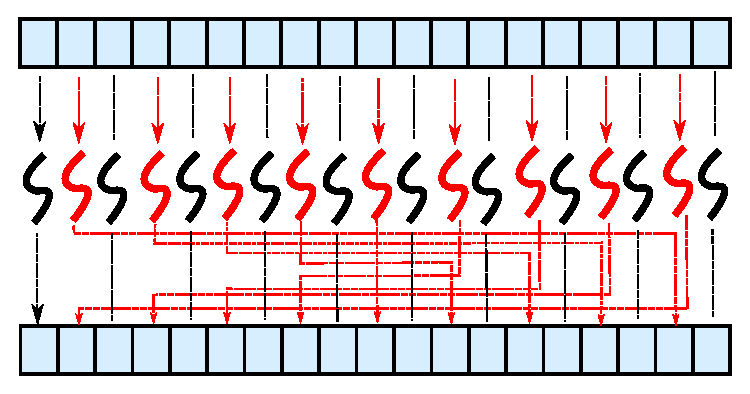
\includegraphics[width=0.9\linewidth]{fig/coalScaleHalf.eps}
\end{minipage}
\begin{minipage}[r]{0.49\linewidth}
  \vspace{1cm}
  \begin{figure}[h]
    \begin{tabular}{|c|c|}
      \hline
      noyau & tps($\mu$s)  \\
      \hline
      contigu & 100 \\
      non-contigu  & 170 \\
      \hline
    \end{tabular}
    \caption{K40M: $N = 2^{20}$}
  \end{figure}
\end{minipage}
  \end{itemize}
\end{frame}

%****************************************************************
% Coalescence
%****************************************************************
\begin{frame}{Quizz}{Tableau de Structures ou Structure de Tableaux}
  \begin{itemize}[<+->]
    \item[\adibi] On veut écrire un noyau qui translate des particules, vaut il mieux utiliser : 
    \item[\galde] un «tableau de structures»
\begin{center}
  \lstinputlisting[language=C]{code/AOS.c}
\end{center}
    \item[\galde] ou une «structure de tableaux»
\begin{center}
  \lstinputlisting[language=C]{code/SOA.c}
\end{center}
  \item[\hand] réponse en TP \pozik
  \end{itemize}
\end{frame}

%****************************************************************
% Déverminage
%****************************************************************
\begin{frame}{Déverminage}{fonctions de l'API}
  \begin{itemize}[<+->]
    \item[\adibi] en C, on {\bf doit} vérifier les retours de fonction 
\begin{center}
  \lstinputlisting[language=C]{code/retour.c}
\end{center}
    \item[\argi] tous les fonctions de l'API CUDA renvoient une \texttt{cudaError\_t}
    \item[\scout] on instrumente le code en mode «DEBUG» grâce à une macro
\begin{center}
  \lstinputlisting[language=C]{code/exErr.c}
\end{center}
  \end{itemize}
\end{frame}

%****************************************************************
% Déverminage
%****************************************************************
\begin{frame}{Déverminage}{fonctions de l'API}
\begin{center}
  \lstinputlisting[language=C]{code/common.h}
\end{center}
\end{frame}

%****************************************************************
% Déverminage : outils I
%****************************************************************
\begin{frame}{Déverminage}{cuda-gdb}
  \begin{itemize}[<+->]
        \item on compile avec les bonnes options \texttt{nvcc -g -G monProg.cu -o myProg}
   \end{itemize}
\pause
  \lstinputlisting[numbers=none,language=bash,basicstyle=\relsize{-5}\ttfamily,lineskip=2pt]{code/outGDB}
\end{frame}

%****************************************************************
% Déverminage : outils I
%****************************************************************
\begin{frame}{Déverminage}{outils}
  \begin{itemize}[<+->]
    \item outil de vérification de mémoire à la «valgrind» : \texttt{cuda-memcheck ./myProg}
    \item[\scout] sinon, pour GPU avec une «capacité de calcul» $\geqslant 2.x$, un bon vieux \texttt{printf} des familles fonctionne aussi
    à l'intérieur d'un noyau \harritu
  \end{itemize} 
\end{frame}

%****************************************************************
% Profilage : 
%****************************************************************
\begin{frame}{Profilage}{API}
  \begin{itemize}[<+->]
    \item[\argi] les évenements CUDA fournissent un moyen simple de mesurer le temps d'execution des noyaux
\begin{center}
  \lstinputlisting[language=C]{code/exProfile.c}
\end{center}
   \item[\kontuz] \texttt{cudaEventElapsedTime} renvoie un temps en milliseconds
   \item[\pozik] on peut scripter {\em en C} des experiences de profilage.
  \end{itemize}
\end{frame}

%****************************************************************
% Profilatzea
%****************************************************************
\begin{frame}{Profilage}{nvprof}
  \begin{itemize}[<+->]
    \item[\pozik] beaucoup plus de métriques et de compteurs disponibles
    \item[\triste] extraction automatique de résultats plus compliquée (merci \texttt{grep})
    \item[\argi] afficher une trace {\tt --print-gpu-trace }
  \end{itemize}
\pause\lstinputlisting[numbers=none,language=bash,basicstyle=\relsize{-5}\ttfamily,lineskip=2pt]{code/outProfile}
\end{frame}

%****************************************************************
% Optimizazio
%****************************************************************
\begin{frame}
  \begin{center}
    {\Huge Seconde partie : Optimization}
  \end{center}
\end{frame}

%****************************************************************
% Limites 
%****************************************************************
\begin{frame}{Facteur limitants}{Petite experience}
  \begin{itemize}[<+->]
    \item soit le noyau \texttt{base} en 3 versions
      \lstinputlisting[language=C]{code/pratique.c}
    \item on chronomètre l'execution (en $\mu$s) avec $N=8Mo$ sur un K40M
      \begin{center}
        \begin{tabular}{|l|r|r|r|}
          \hline
          modèle    & base    & memory & math  \\ 
          \hline
          normal    &  618    &  390   &  473\\ 
          fastmath  &  546    &  390   &  385 \\ 
          \hline
        \end{tabular}
      \end{center}
  \end{itemize}
\end{frame}

%****************************************************************
% mugatzaileak
%****************************************************************
\begin{frame}{Facteur limitants}{Mémoire, instruction ou latence}
  \begin{itemize}[<+->]
    \item limitation par les {\bf instructions} (compute bound) 
      \begin{itemize}
        \item sans {\tt fastmath} : utilisation préponderante du calcul
      \end{itemize}
    \item limitation par la {\bf mémoire } (memory bound) : 
      \begin{itemize}
        \item avec {\tt fasthmath} facteur mémoire préponderant
      \end{itemize}
    \item limitation par la {\bf latence} : utilisation faible de la mémoire et des calculs
      \begin{itemize}
        \item possibilité d'une {\bf occupation} faible 
          $$ \mbox{Occupation} = \frac{\mbox{nb de chaînes(warps) actives par SM}}{\mbox{nb max de chaînes par SM}} $$
      \begin{itemize}
        \item théorique : {\tt cudaOccupancyMaxActiveBlocksPerMultiprocessor }
        \item réelle : {\tt nvprof --metrics achieved\_occupancy }
      \end{itemize}
        \item calage des threads (dépendance d'executions, synchronisation, chargement d'instruction)
      \end{itemize}
\end{itemize}
\end{frame}

%****************************************************************
% facteur limitants
%****************************************************************
\begin{frame}{Bande Passante(BP)}
  \begin{itemize}[<+->]
    \item débit de données en Go/s sur le bus mémoire du GPU 
    \item BP max théorique : $$BW_{\mbox{max}} = 2 \cdot \frac{F_{\mbox{max}} * N_{\mbox{bus}}}{10^6} $$
      \begin{itemize}
        \item $F_{max}$ : fréquence mémoire maximale (KHz) : \texttt{memoryClockRate}
        \item $N_{bus}$ : largeur de bus (octets) : \texttt{memoryBusWidth}/8
      \end{itemize}
    \item BP réelle d'un noyau : $$ BW_{\mbox{ker}} = \frac{\# R_{\ker} + \# W_{\ker}}{10^9 t_{\ker}} $$
      \begin{itemize}
        \item $\# R_{\ker}$ : nb de lectures du noyau (octets)
        \item $\# W_{\ker}$ : nb d'ecritures du noyau (octets)
        \item $t_{\ker}$ : tps moyen d'exécution du noyau
      \end{itemize}
  \end{itemize}
\end{frame}

%****************************************************************
% Performances 
%****************************************************************
\begin{frame}{Quelques performances}
  \begin{itemize}[<+->]
    \item la capacité de calcul (CC) dépend de l'architecture
    \item Flops = $\frac{Flops}{cycle}\times \mbox{\#cœurs} \times \frac{\mbox{cycle}}{\mbox{seconde}} \approx
         2\footnote{https://en.wikipedia.org/wiki/FLOPS} \times \mbox{\#cœurs} \times \mbox{Freq} $
       \item si (CC)  $\nearrow$ , le nombre de GFlops\; $\nearrow$ aussi \pozik
  \end{itemize}
\pause
 \begin{tabular}{|l|r|r|r|r|r|r|}
    \hline
      modèle         & C1060   & C2070 &  K40   &  M40    &  P100  & V100  \\
    \hline
      archi          & Tesla   & Fermi & Kepler & Maxwell & Pascal & Volta \\
      CC             & 1.3     & 2.0   & 3.5    & 5.2     & 6.0    &   7.0 \\
      Freq(Mhz)      & 1296    & 1150  &  745   &  1114   &  1329  &  1380 \\
      SM             & 30      & 14    &  15    &  24     &   56   &   80  \\
      SP (32)        & 240     & 448   &  2880  &  3072   &  3584  &  5120 \\
      Flops (G/s)    & 622     & 1030  &  4291  &  6844  & 9526   &  14131\\
      BP$_{max}$ (Go/s) & 102     & 150   &  288   &  288    & 732    &  790 \\
    \hline
\end{tabular}
\end{frame}

%****************************************************************
% facteur limitants
%****************************************************************
\begin{frame}{Facteur limitants}{bande passante}
  \begin{itemize}[<+->]
    \item en revenant a l'exemple précedents ( tps \gezi\ BP)
      \begin{center}
        \begin{tabular}{|l|r|r|r|}
          \hline
          modèle  & base   & memory & math  \\ 
          \hline
          normal  &  108    &  172   &  141 \\ 
          fastmath  &  122    &  172   &  174 \\ 
          \hline
        \end{tabular}
      \end{center}
     \item à comparer avec la valeur max théorique de 288 Go/s!
  \end{itemize}
\end{frame}

%****************************************************************
% transferentziak
%****************************************************************
\begin{frame}{Transferts Hôte \geziBikoitz\  GPU}{Ordres de grandeur}
  \begin{itemize}[<+->]
    \item[\argi] BP DRAM GPU \geziBikoitz\ SMs $\thicksim$ 200-300 (Go/s)
    \item[\argi] BP Mémoire Globale \geziBikoitz\ DRAM GPU $\thicksim$ 10-20 (Go/s)
    \item[\scout] il faut donc optimiser les transferts hôte \geziBikoitz\ GPU
      \begin{itemize}
        \item mémoire verrouillée
        \item transferts asynchrones
      \end{itemize}
    \item[\kontuz] on a beau avoir le noyau le plus rapide du monde, si le temps de transfert est prohibitif, ça ne sert à rien \harritu
  \end{itemize}
\end{frame}

%****************************************************************
% memoria giltzatuta
%****************************************************************
\begin{frame}{Mémoire vérrouillée}
  \begin{itemize}[<+->]
    \item[\argi] allocation par défaut \gezi\ mémoire paginable (pouvant utiliser l'espace d'échange)
    \item[\argi] transfert \geziBikoitz\  GPU
      \begin{itemize}
        \item contrôleur DMA choisit : paginable ou verrouillée
        \item la mémoire verrouillée interdit l'utilisation du «swap»
        \item l'usage de la mémoire paginable nécessite d'abord l'allocation d'un tampon verrouillé, puis une copie vers le GPU
      \end{itemize}
  \end{itemize}
\pause
  \begin{center}
  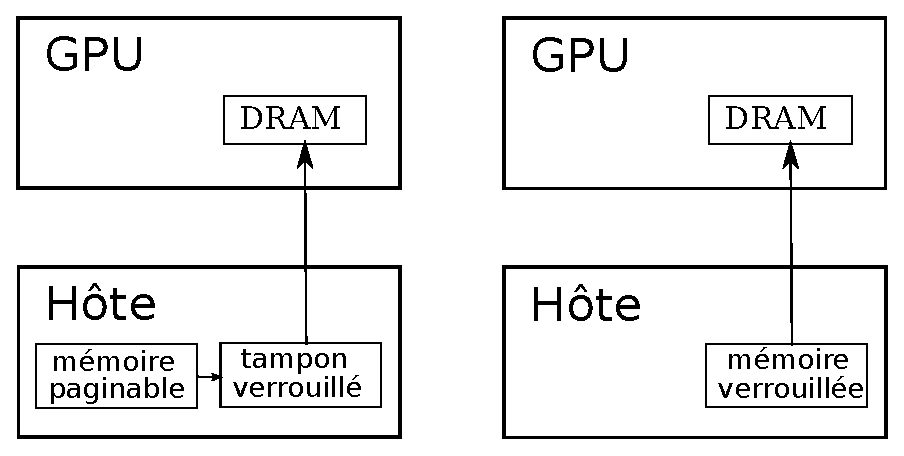
\includegraphics[width=0.6\linewidth]{fig/pinned_memory.eps}
  \end{center}
\end{frame}
%****************************************************************
% memoria giltzatuta
%****************************************************************
\begin{frame}{Mémoire vérrouillée}{exemple}
  \begin{itemize}[<+->]
    \item[\argi] allocation {\tt cudaHostAlloc}, desallocation {\tt cudaFreeHost}
    \item[\argi] ou enregistrement de mémoire deja alloué par {\tt malloc} avec {\tt cudaHostRegister}
  \lstinputlisting[language=C]{code/pinned.c}
\item[\argi] on peut utiliser aussi de la mémoire associée (cudaHostAllocDefault \gezi\ cudaHostAllocMapped) pour éviter la recopie, mais la BP est moins rapide depuis les noyaux
\item[\triste] gain faible (ex sur un k40M 8.9Go/s vs 7Go/s pour 32M)
  \end{itemize}
\end{frame}
%****************************************************************
% transfert asynchrones
%****************************************************************
\begin{frame}{Transferts asynchrones}{Principe}
  \begin{itemize}[<+->]
    \item[\kontuz] les transferts classiques (ex {\tt cudaMemcpy}) sont {\bf bloquants} \harritu
\begin{center}
  
\includegraphics[width=0.6\linewidth]{fig/seq.png}
\end{center}
    \item[\scout] utiliser des transferts {\bf asynchrones } pour recouvrir les transferts par des calculs
\begin{center}
  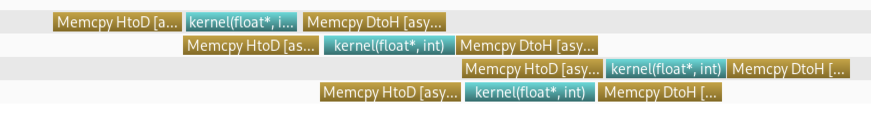
\includegraphics[width=0.95\linewidth]{fig/async.png}
\end{center}
    \item[\argi] répartir les données sur des {\bf flux} («streams») différents
    \item[\kontuz] la mémoire sur l'hôte doit être vérouillée
    \item[\pozik] le pipeline de transfert de données permet un recouvrement \\ 
      \gezi\ réduction du temps total
  \end{itemize}
\end{frame}

%****************************************************************
% transfert asynchrones : exemple
%****************************************************************
\begin{frame}{Transferts asynchrones}{Exemple}
  \begin{itemize}[<+->]
    \item[\adibi] sur d'un noyau 1D 
      \lstinputlisting[language=C]{code/asyn.c}
    \item[\faClockO] sur K40M, avec N=4Mo et 4 flux \\ \gezi\ 4.71ms (sequentiel) vs 2.67ms (asynchrone) \pozik
  \end{itemize}
\end{frame}

%****************************************************************
% Mémoires de l'accelerateur
%****************************************************************
\begin{frame}{Mémoires sur l'accélérateur}{Vue générale}
  \begin{itemize}[<+->]
    \item[\argi] un GPU abrite plusieurs types de mémoire : 
\begin{tabular}{|l|l|l|l|l|l|}
  \hline
  mémoire   & local. & Cachée  & accès     & portée   & durée \\ 
  \hline
  registre  & puce  &  N/A   & RW & thread & thread \\
  locale    & DRAM  & CC$\geqslant$2.0 & RW & thread & thread \\
  partagée  & puce  & N/A    & RW & bloc   & bloc \\
  globale   & DRAM  & CC$\geqslant$2.0  & RW & GPU et hôte &  appli. \\
  constante & DRAM  & Oui    & R  & GPU et hôte &  appli. \\
  texture   & DRAM  & Oui    & R  & GPU et hôte &  appli. \\
  \hline
\end{tabular}
  \item[\kontuz] différentes caractéristiques \gezi\ différents usages
    \begin{itemize} 
     \item la mémoire constante permet de «cacher» des données constantes durant l'execution du noyau, mais ses
       accès doivent être constants par thread 
     \item la mémoire partagée permet d'avoir un cache local pour un bloc de threads
  \end{itemize}
  \end{itemize}
\end{frame}

%****************************************************************
% mémoire partagée : 
%****************************************************************
\begin{frame}{Mémoire partagée}
  \begin{itemize}[<+->]
    \item[\argi] mémoire partagée entre tous les threads d'un bloc
    \item[\kontuz] aux écritures concurrentes \harritu
    \item[\scout] synchronisation à l'aide de {\tt \_\_syncthreads } 
    \item[\scout] déclaration à l'aide du mot-clef {\tt \_\_shared\_\_}
    \item[\scout] allocaton statique...
  \lstinputlisting[language=C]{code/sharedStatic.c}
\item[\scout] ou dynamique
  \lstinputlisting[language=C]{code/shareDynamic.c}
   \item[\kontuz] taille limitée à 64kB
   \end{itemize}
\end{frame}

%****************************************************************
% mémoire partagée : exemple
%****************************************************************
\begin{frame}{Mémoire partagée}{Tranposition}
  \begin{itemize}[<+->]
    \item[\adibi] on considère un noyau qui transpose une matrice
  \lstinputlisting[language=C]{code/transposeNaive.c}
    \item[\triste] écriture avec un saut de longueur {\tt n.x }\gezi\ non coalescent \harritu
\begin{center}
  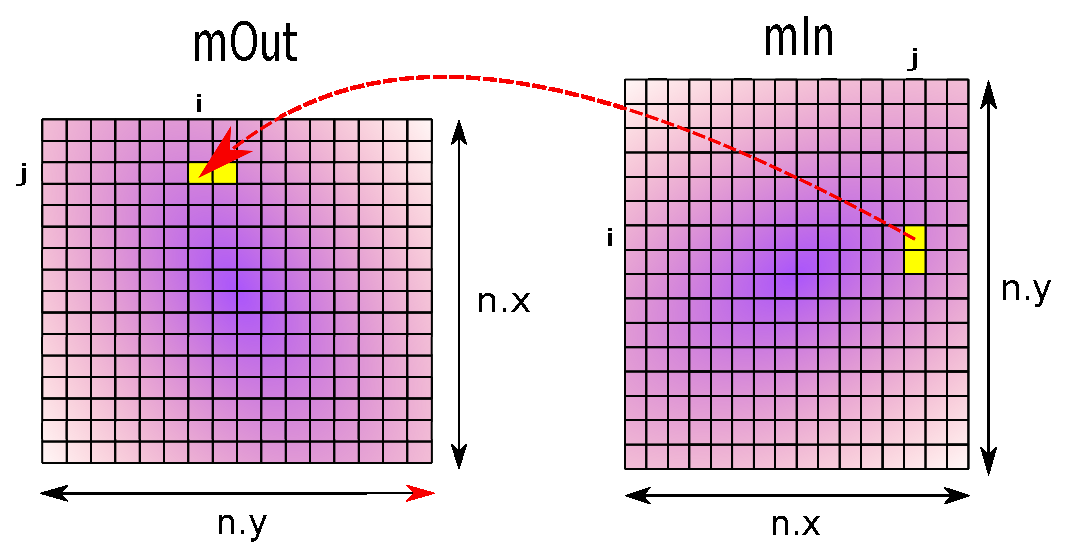
\includegraphics[width=0.7\linewidth]{fig/transpose1.eps}
\end{center}
   \end{itemize}
\end{frame}

%****************************************************************
% mémoire partagée : solution
%****************************************************************
\begin{frame}{Mémoire partagée}{solution}
  \begin{itemize}[<+->]
    \item[\argi] on utilise un cache local \gezi\ lecture coalescente \pozik
  \lstinputlisting[language=C]{code/transposeShared1.c}
\begin{center}
  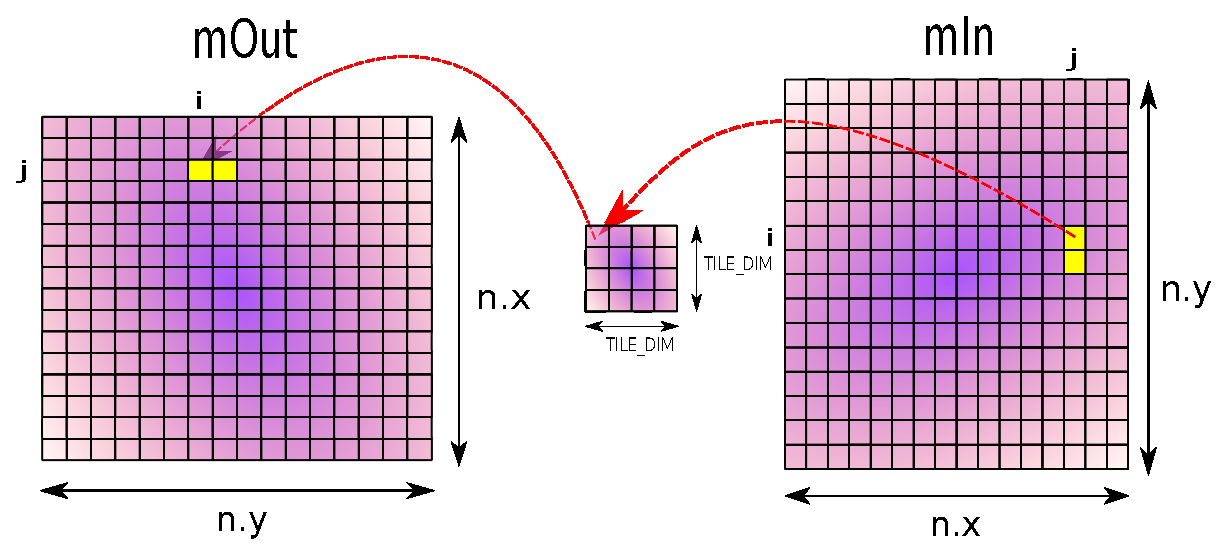
\includegraphics[width=0.60\linewidth]{fig/transpose2.eps}
\end{center}
   \item[\faMagic] tester {\tt \_\_shared\_\_ float tile[TILE\_DIM][TILE\_DIM+1]} 
   \end{itemize}
\end{frame}

%****************************************************************
% mémoire partagée : synchronisation
%****************************************************************
\begin{frame}{Mémoire partagée}{sur l'importance de la synchonisation}
 \begin{itemize}[<+->]
   \item on veut transposer l'image suivante
\begin{center}
  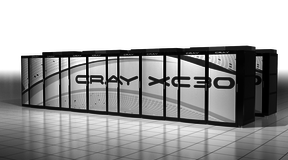
\includegraphics[width=0.4\linewidth]{fig/cray.png}
\end{center}
  \item[\faClockO] image 2976x3808 sur K40M \gezi\ 0.94ms vs 0.75ms 
\end{itemize}
\pause
\begin{columns}[t]
\column{5cm}
 Sans synchronisation 
\begin{center}
  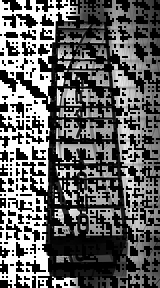
\includegraphics[width=0.3\linewidth]{fig/crayNoSync.png}
\end{center}
\column{5cm}
 Avec synchronisation
\begin{center}
  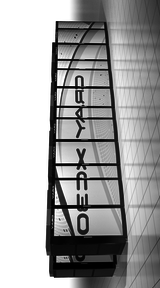
\includegraphics[width=0.3\linewidth]{fig/crayTrans.png}
\end{center}
\end{columns}
\end{frame}

%****************************************************************
% Divergence de thread
%****************************************************************
\begin{frame}{Divergence de chaînes}
 \begin{itemize}[<+->]
  \item[\kontuz] la divergence de chaîne peut degrader les performances
  \item[\adibi] soit le noyau suivant
  \lstinputlisting[language=C]{code/warpDiverge.c}
  \item[\argi] condition satisfaite par 1 thread d'une chaîne 
    \begin{itemize}
      \item[\gezi] {\bf tous} les threads de la chaîne executent cette branche
      \item[\gezi] les autres branches d'exécution sont serialisées
      \item[\gezi] masquage des résultats des threads hors branche
    \end{itemize}
  \item[\adibi] par contre le noyau suivant ne diverge pas
  \lstinputlisting[language=C]{code/warpNoDiverge.c}
  \end{itemize}
\end{frame}

%****************************************************************
% Redukzio : Monte-Carloko metodoa
%****************************************************************
\begin{frame}{Réduction}{Calcul de $\pi$ par une méthode de Monte-Carlo}
 \begin{itemize}[<+->]
   \item[\argi] On souhaite approcher $\pi$ par le calcul d'aire suivant
     \begin{columns}
       \column{6cm}
\begin{center}
  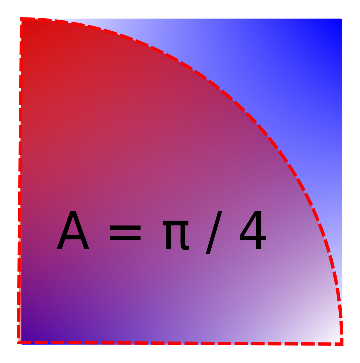
\includegraphics[width=0.5\linewidth]{fig/monteCarlo.eps}
\end{center}
       \column{4cm}
  $$A = \int_{A} dx \thicksim \frac{1}{N}\sum_{i=1}^N \mathbb{1}_{A}(x_i)$$
     \end{columns}
 où les $x_i$ sont pris au hasard dans le carré $[0,1] \times [0,1]$
  \item[\faBomb] méthodes dite «de Monte-Carlo» en réference à l'algorithme de Metropolis-Ulam \gezi\ pendant info. de l'aiguille de Buffon
  \item[\triste] convergence lente en $O(\frac{1}{\sqrt{N}})$
  \item[\pozik] massivement parallélisable si on a un générateur pseudo-aléatoire parallèle (\texttt{curandGenerateUniform})
  \end{itemize}
\end{frame}


%****************************************************************
% Redukzio : Somme
%****************************************************************
\begin{frame}{Réduction}{Principe}
 \begin{itemize}[<+->]
   \item[\argi] générer en // des couples aléatoires $(x_i,y_i) \in K = [0,1]^2$
   \item[\argi] sommer en // ceux qui sont dans $A = \{ (x,y) \in K \;|\; x^2+y^2 \geqslant 1 \}$
   \item[\galde] comment calculer une somme en parallèle sur un GPU ?
   \item[\kontuz] il faut faire travailler un max de threads \harritu
   \item[\scout] par exemple, en utilisant une réduction en arbre 
  \end{itemize}
\pause
\begin{center}
  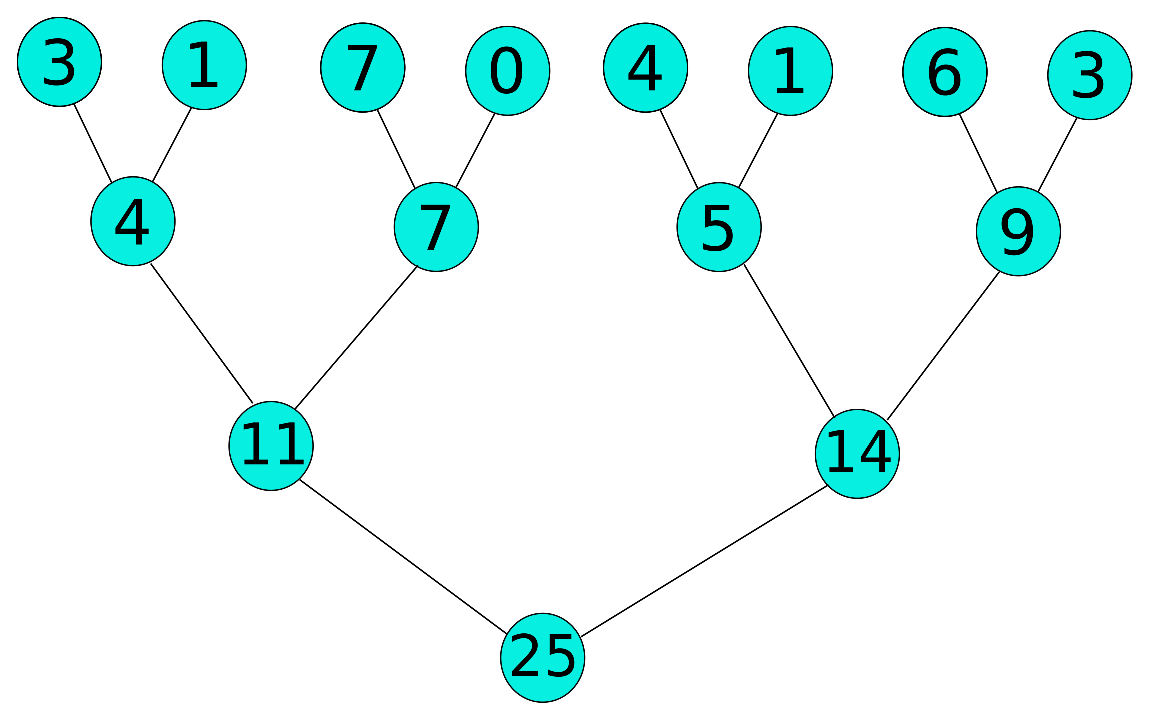
\includegraphics[width=0.6\linewidth]{fig/zuhaitz.eps}
\end{center}
\end{frame}

%****************************************************************
% Redukzio : Somme
%****************************************************************
\begin{frame}{Réduction}{2 niveaux} 
 \begin{itemize}[<+->]
   \item[\scout] On va écrire 2 noyaux, qu'on appelle en cascade
 \begin{enumerate}
   \item {\tt partialSum} qui dénombre les couples $(x_i,y_i)$ dans $A$ pour chaque bloc. 
   \item stockage du résultat en mémoire globale ({\tt partial})
   \item {\tt finalSum} calcule la somme des éléments de {\tt partial}
 \end{enumerate}
   \item[\kontuz] information commune par bloc \gezi\ mémoire partagée
   \item[\argi] schéma d'appel
     \lstinputlisting[language=C]{code/biKernels.c}
     \begin{center}  
  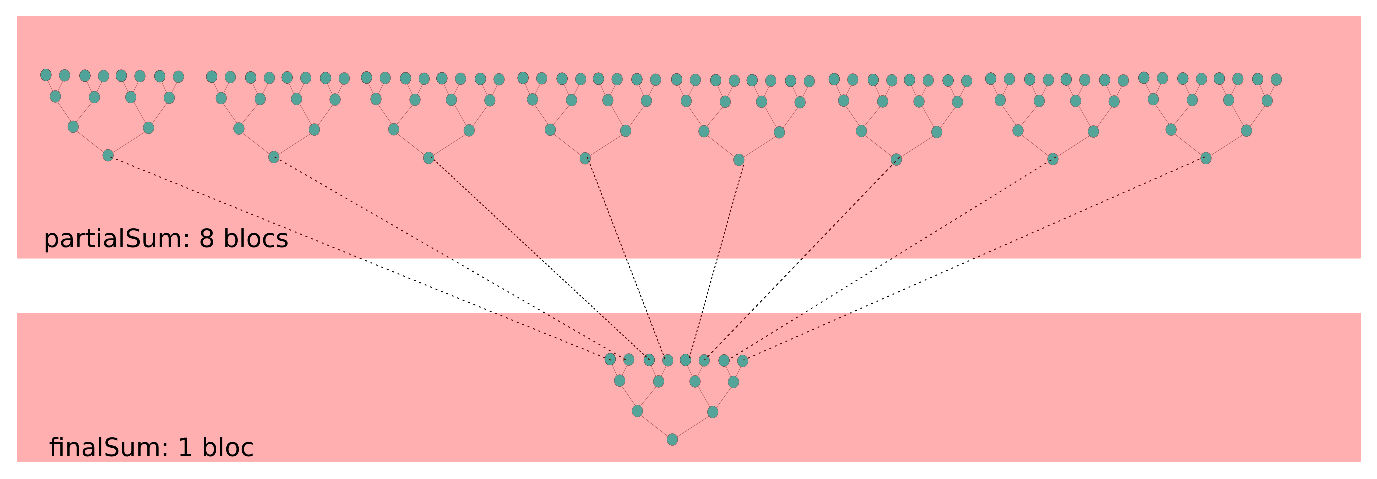
\includegraphics[width=0.6\linewidth]{fig/biKernels.eps}
     \end{center}  
   \item[\argi] écriture possible avec un seul noyau \gezi\ opérations {\em atomiques}
  \end{itemize}
 \end{frame}

%****************************************************************
% Redukzio : somme divergente
%****************************************************************
\begin{frame}{Réduction}{Première solution}
 \begin{enumerate}[<+->]
   \item On peut ajouter 2 cases mémoire contiguës
   \item multiplier le pas par 2
   \item et itérer...
  \end{enumerate}
\pause
\begin{center}
  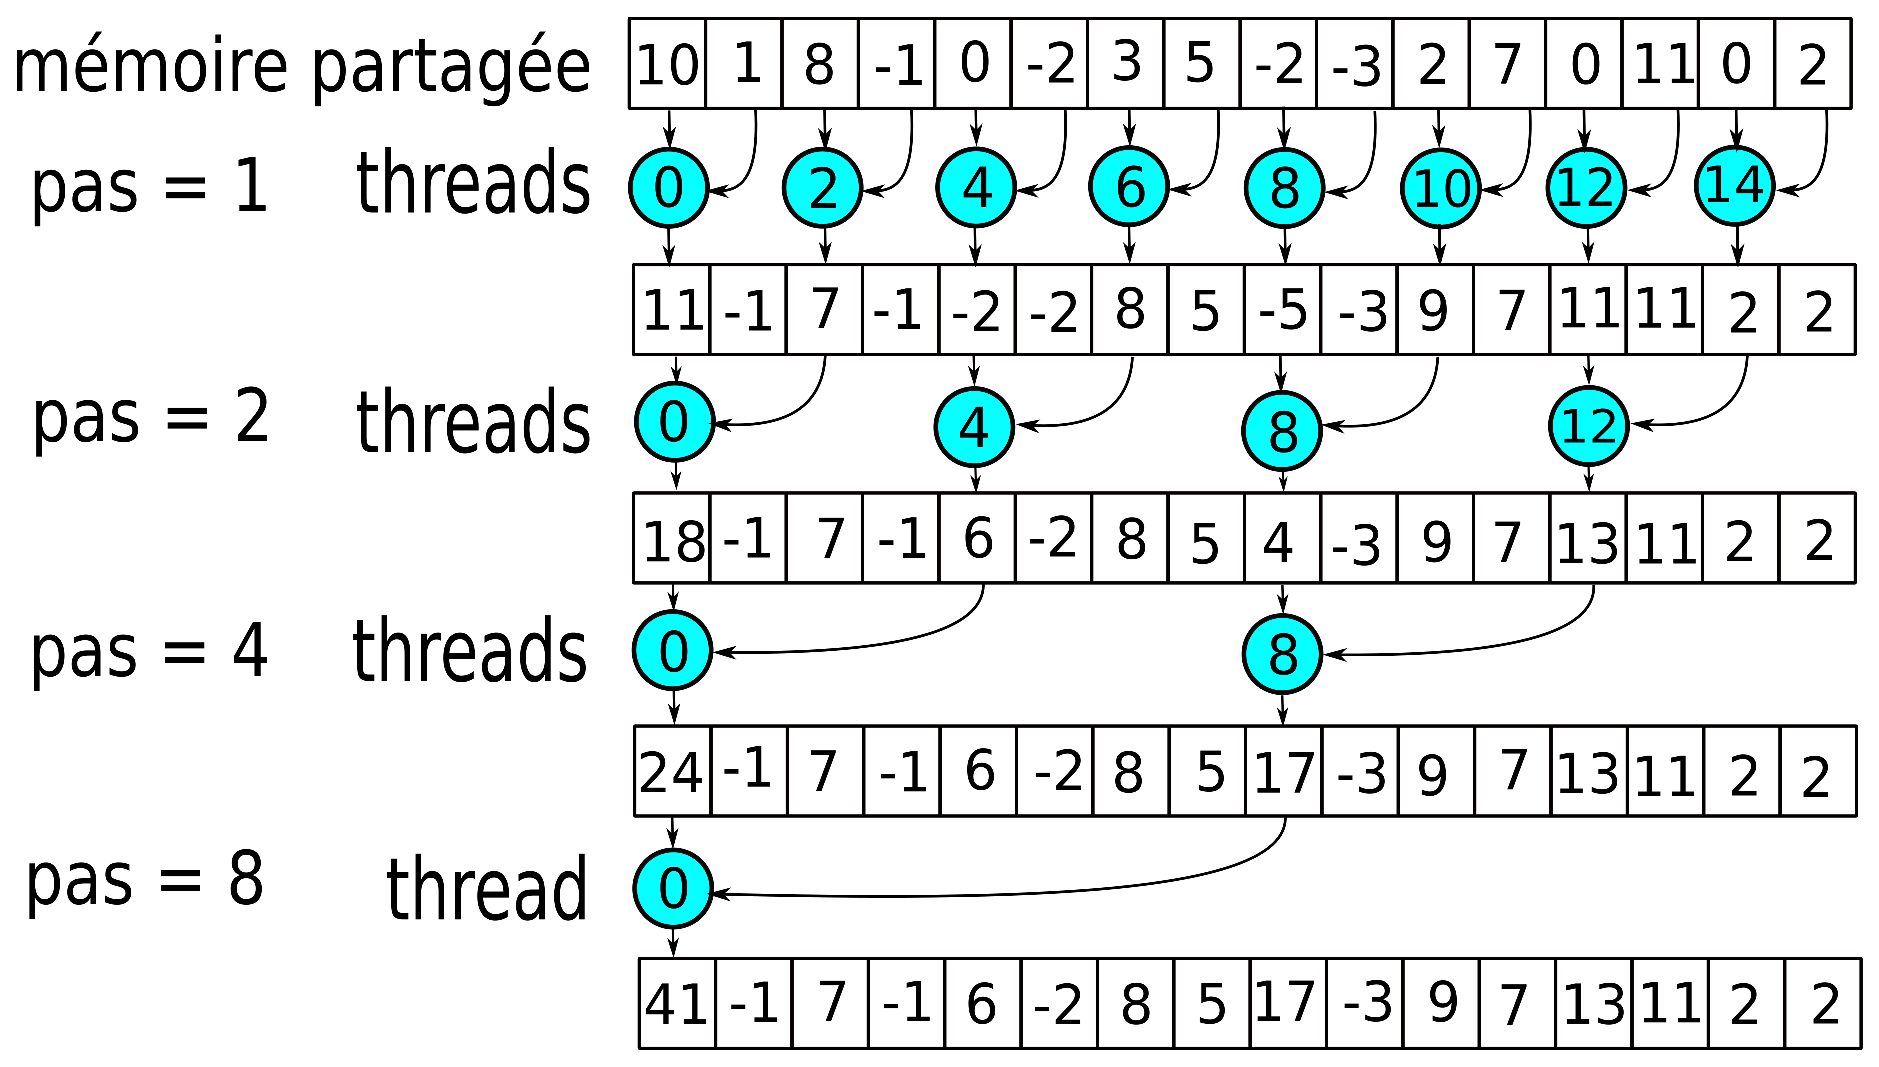
\includegraphics[width=0.8\linewidth]{fig/divergent.eps}
\end{center}
\pause
\begin{itemize}
  \item[\triste] problème : le schéma est clairement divergent \harritu
  \end{itemize}
\end{frame}

%****************************************************************
% Redukzio : somme convergente
%****************************************************************
\begin{frame}{Réduction}{2$^{\mbox{ème}}$ solution}
 \begin{enumerate}[<+->]
   \item ou alors additioner avec l'element situé a {\tt blockDim.x}
   \item et diviser le pas par 2
   \item puis itérer...
  \end{enumerate}
\pause
\begin{center}
  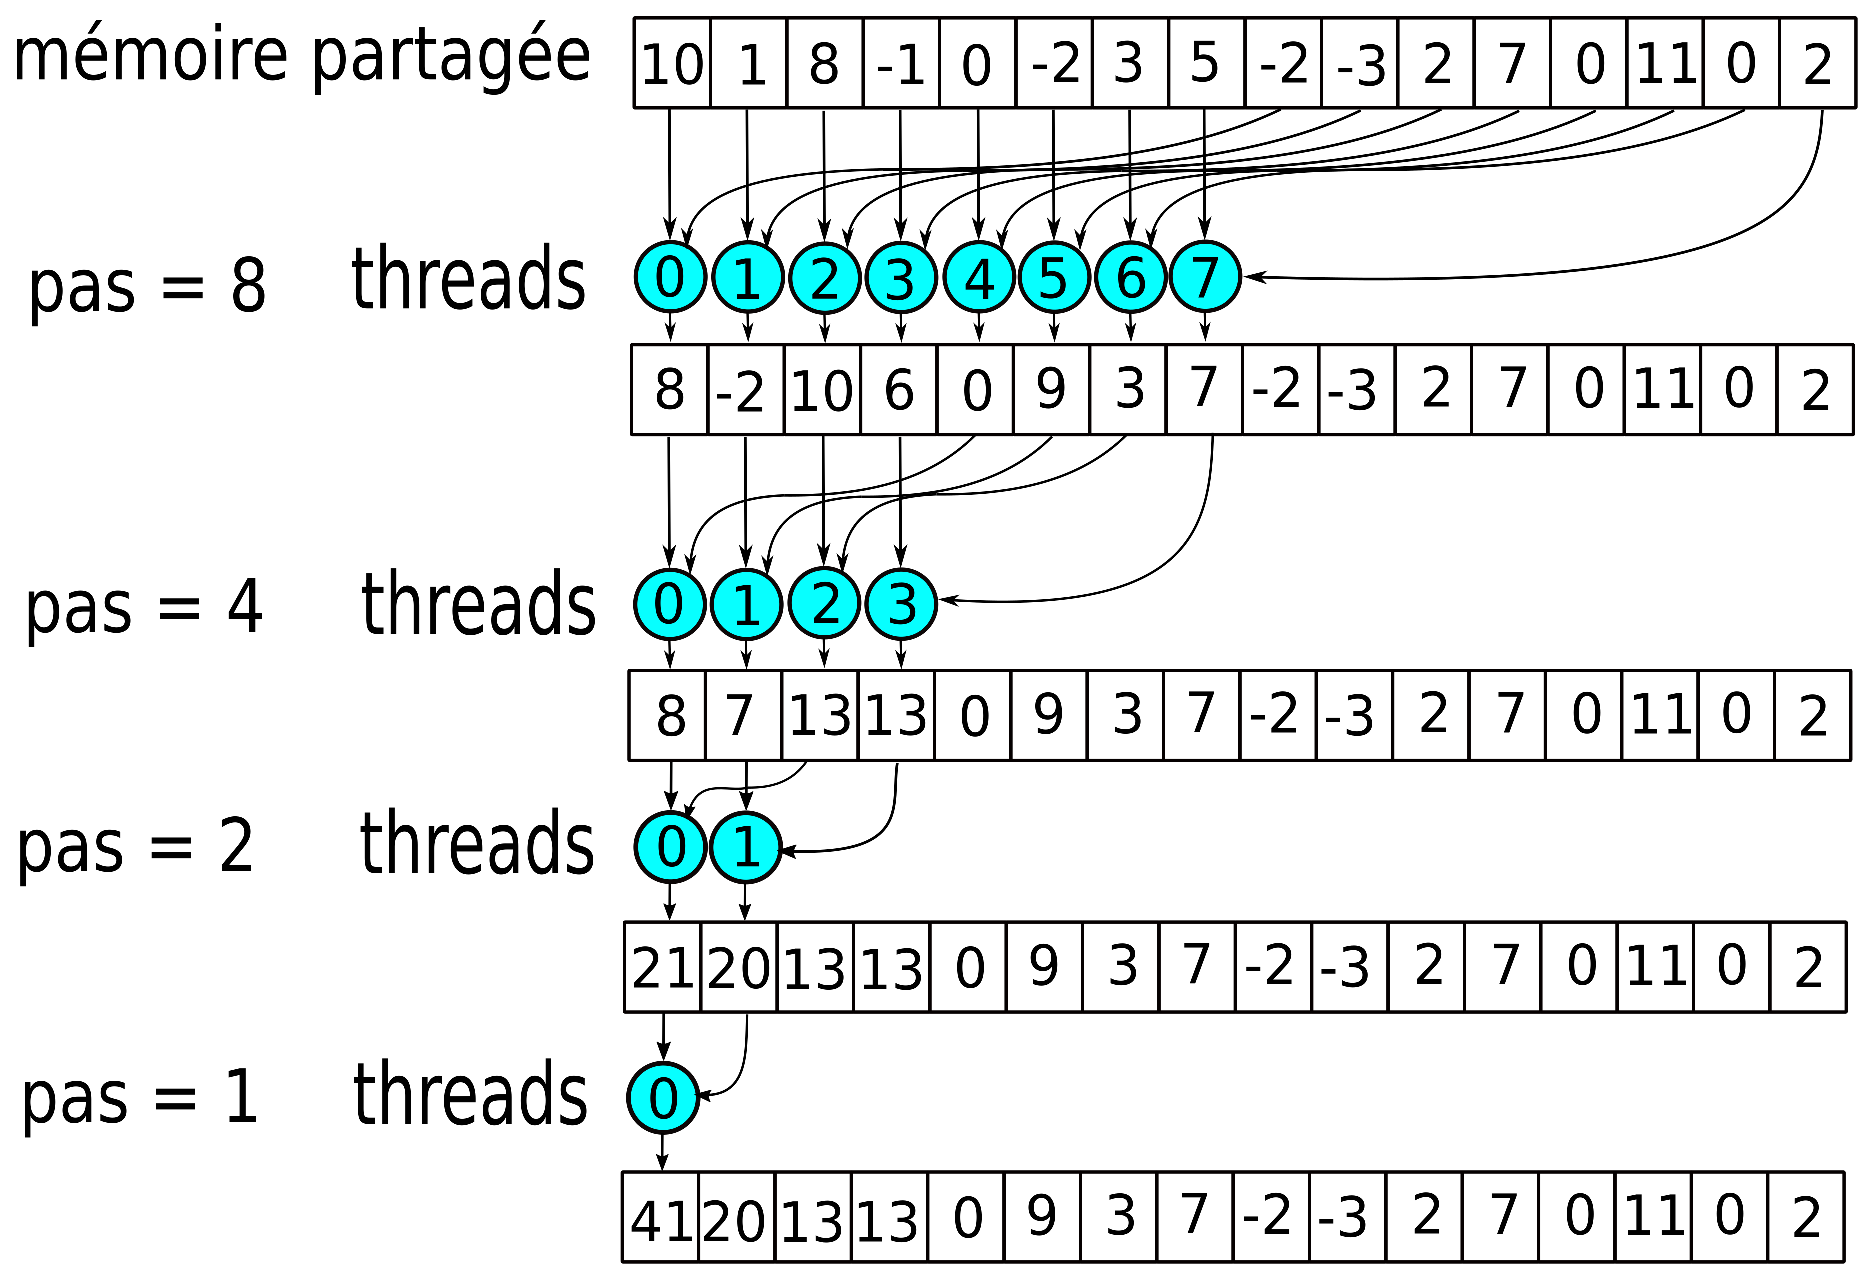
\includegraphics[width=0.6\linewidth]{fig/convergent.eps}
\end{center}
\pause
\begin{itemize}
  \item[\pozik] le schéma ne diverge quasiment plus \harritu
  \end{itemize}
\end{frame}

%****************************************************************
% Divergence de thread
%****************************************************************
\begin{frame}{Réduction}{noyau «partialSum»}
\pause
  \lstinputlisting[language=C]{code/partialSum.c}
\pause
  \begin{itemize}[<+->]
    \item chaque thread traite $\lfloor \frac{N}{\mbox{{\tt gridDim.x * blockDim.x}}}\rfloor $ données
    \item synchro multiple
    \item {\tt psum} : tableau partagé de taille {\tt BLOCK\_SIZE }
    \item {\tt finalSum} a un code trés similaire
  \end{itemize}
\end{frame}

%****************************************************************
% hirurgarren partea : denetarik
%****************************************************************
\begin{frame}
  \begin{center}
    {\Huge $3^{\mbox{ème}}$ partie : Divers }
  \end{center}
\end{frame}

%****************************************************************
% gpu-ri buruzko historio motz bat
%****************************************************************
\begin{frame}{Une brève histoire des GPUs}{Les premiers âges}
  \begin{columns}[t]
    \column{7cm}
    \begin{itemize}[<+->]
      \item bonne synthèse sur \href{https://www.techspot.com/article/650-history-of-the-gpu/}{\beamergotobutton{Techspot}}
      \item premiers coprocesseurs graphiques évidemment qu'en 2D
        \begin{itemize}
          \item 1976 : RCA Pixie (résolution 62x128)
          \item 1977 : Adaptateur d'interface de Télevision TIA 1A (Atari 2600)
          \item 1981 : Motorola MC6845 (IBM PC, Apple II)
        \end{itemize}
    \end{itemize}
    \column{5cm}
    \begin{figure}[htbp]
  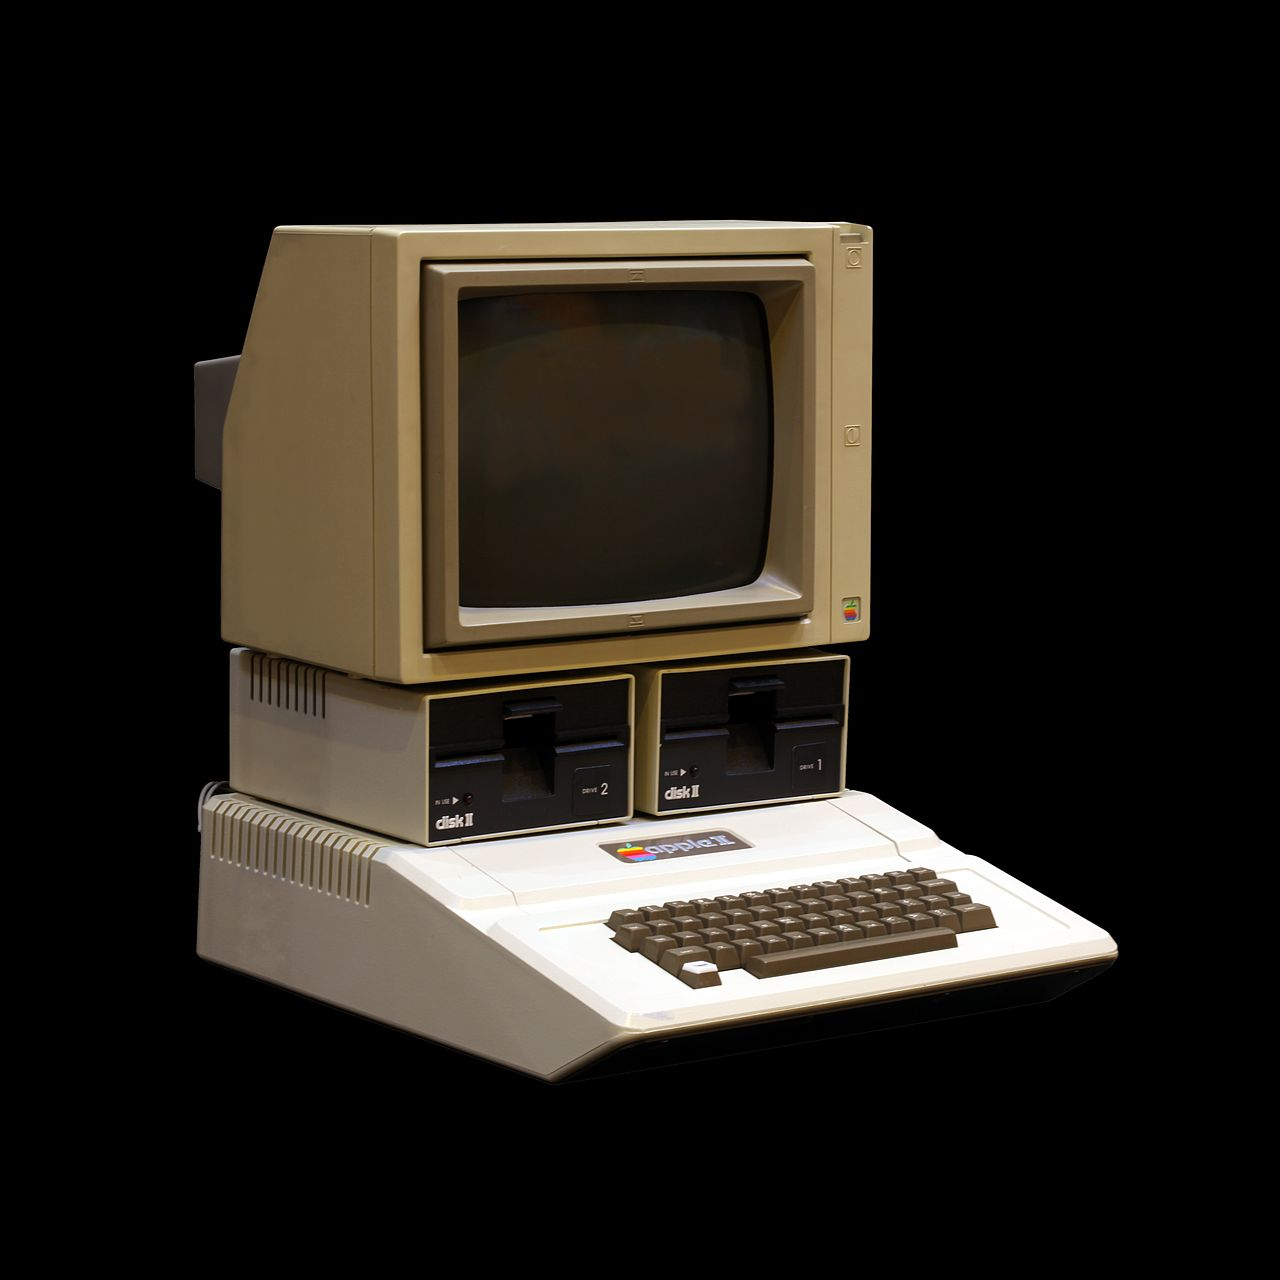
\includegraphics[width=0.8\linewidth]{fig/appleII.jpg}
    \caption{\tiny Apple IIe : 560x192 en monochrome, 15 couleurs en 140x192 !}
    \end{figure}
  \end{columns}
\end{frame}


%****************************************************************
% souvenirs, souvenirs
%****************************************************************
\begin{frame}{Souvenirs, souvenirs}{Lode Runner sur Apple IIe}
  \begin{center}
  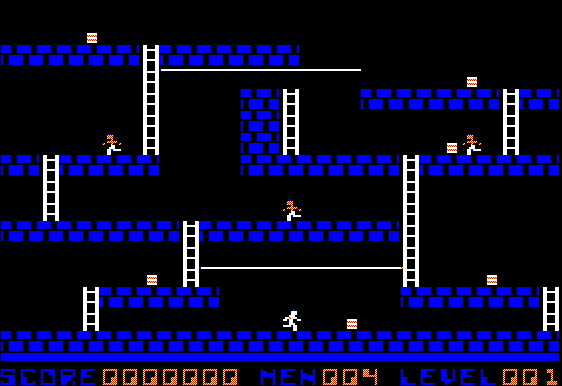
\includegraphics[width=0.8\linewidth]{fig/lode_runner.png}
  \end{center}
\end{frame}

%****************************************************************
% gpu-ri buruzko historio motz bat
%****************************************************************
\begin{frame}{Une brève histoire des GPUs}{les premiers âges}
  \begin{columns}[t]
    \column{7cm}
    \begin{itemize}[<+->]
     \item 1983: Intel iSBX 275 Video Graphics 
    Controller Multimode Board
    \begin{itemize}
      \item 256x256, 8 colors
  \item 512x512 monochrome
  \item Lignes, rectangles, cercles...
  \item zoom \& défilement matériels
  \item 32KB, 1000\$ \harritu
  \item simulateurs de vol (Armée)
    \end{itemize} 
    \item 1987: ATI EGA
      \begin{itemize}
        \item 650x350, 16 couleurs
        \item 512x512 monochrome
        \item 256KB de DRAM
        \item 399\$ \pozik
        \item EGA Wonder 800
        \begin{itemize}
          \item  800x600 VGA
          \item  449\$
        \end{itemize} 
      \end{itemize} 
   \end{itemize} 
    \column{5cm}
    \begin{figure}[htbp]
  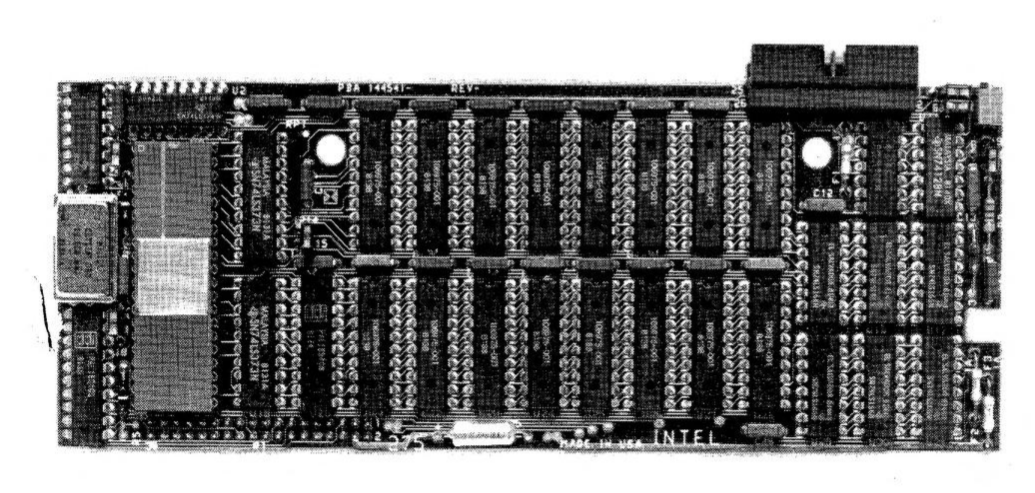
\includegraphics[width=0.8\linewidth]{fig/sbx2.png}
      \caption{\tiny iSBX 275}
    \end{figure}
\begin{figure}[htbp]
  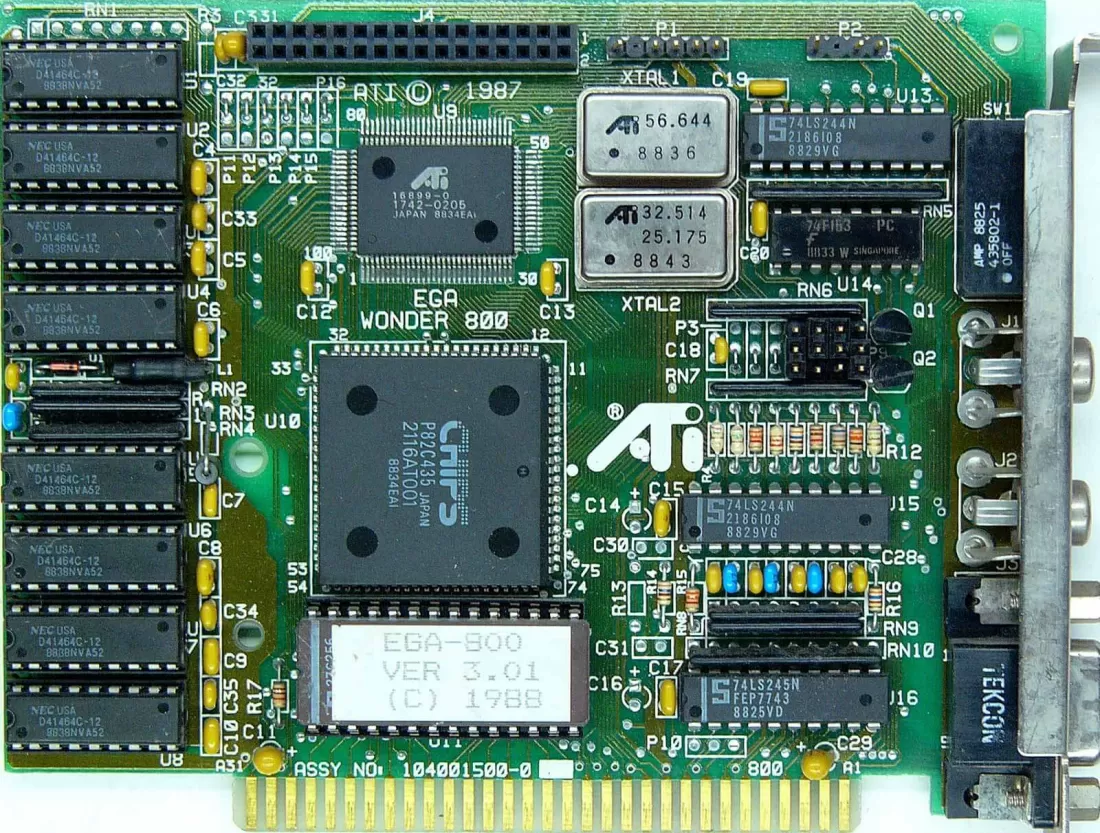
\includegraphics[width=0.8\linewidth]{fig/ati_ega.png}
      \caption{\tiny ATI EGA Wonder 800}
    \end{figure}
  \end{columns}
\end{frame}

%****************************************************************
% gpu-ri buruzko historio motz bat
%****************************************************************
\begin{frame}{Une brève histoire des GPUs}{les premiers âges}
  \begin{columns}[t]
    \column{7cm}
    \begin{itemize}[<+->]
      \item 1992 : SGI publie OpenGL 1.0 
        \begin{itemize}
          \item Interface de Programmation Applicative (IPA) pour 
            la 2D et 3D.
         \item initialement prévu pour Uni
         \item vite adopté pour les jeux 3D
         \end{itemize}
      \item 1992: Wolfenstein 3D (Id Software)
        \begin{itemize}
          \item un des premiers FPS (jeux de tir en vue subjective)
            \href{https://classicreload.com/wolfenstein-3d.html}{\beamergotobutton{Jouer}}
         \end{itemize}
      \item 1993: naissance de Nvidia
      \item 1995: Microsoft promeut son IPA Direct3D 
    \end{itemize} 
    \column{5cm}
\begin{figure}[htbp]
  
\includegraphics[width=0.7\linewidth]{fig/opengl.png}
 \end{figure}
\begin{figure}[htbp]
  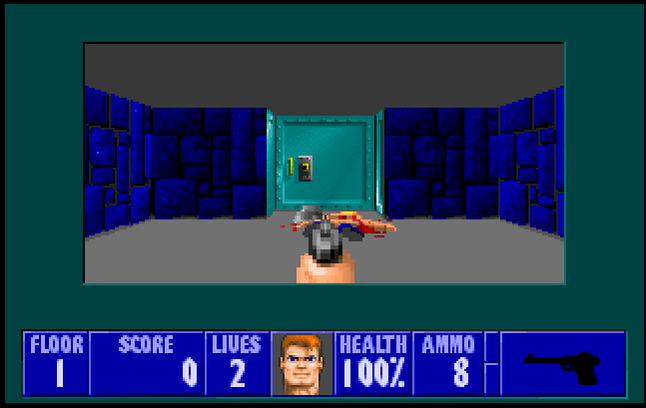
\includegraphics[width=0.8\linewidth]{fig/wolf2.png}
    \end{figure}
  \end{columns}
\end{frame}

%****************************************************************
% gpu-ri buruzko historio motz bat
%****************************************************************
\begin{frame}{Une brève histoire des GPUs}{ou comment la 3dfx Voodoo change la donne}
  \begin{columns}[t]
    \column{7cm}
    \begin{itemize}[<+->]
      \item 1995 : IPA Glide publié par 3dfx interactive
        \begin{itemize}
         \item sous-ensemble de OpenlGL 1.1
         \item placage de texture
         \end{itemize}
      \item 1995 : Nvidia NV1 : premiere puce integrant
        \begin{itemize}
          \item rendu 3D
          \item accélération vidéo
         \end{itemize}
      \item 1996 : 3dfx voodo Graphics
        \begin{itemize}
          \item uniquement 3D, IPA Glide
          \item application phare : Quake (ID software)
        \end{itemize} 
    \end{itemize} 
    \column{5cm}
\begin{figure}[htbp]
  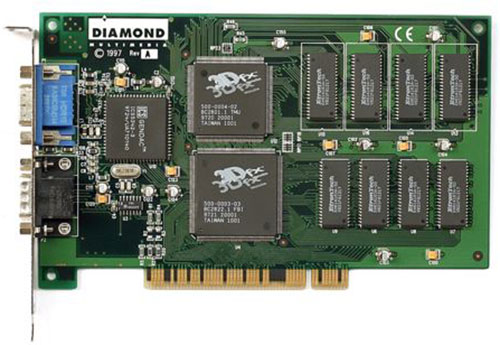
\includegraphics[width=0.7\linewidth]{fig/3dfx.jpg}
 \end{figure}
\begin{figure}[htbp]
  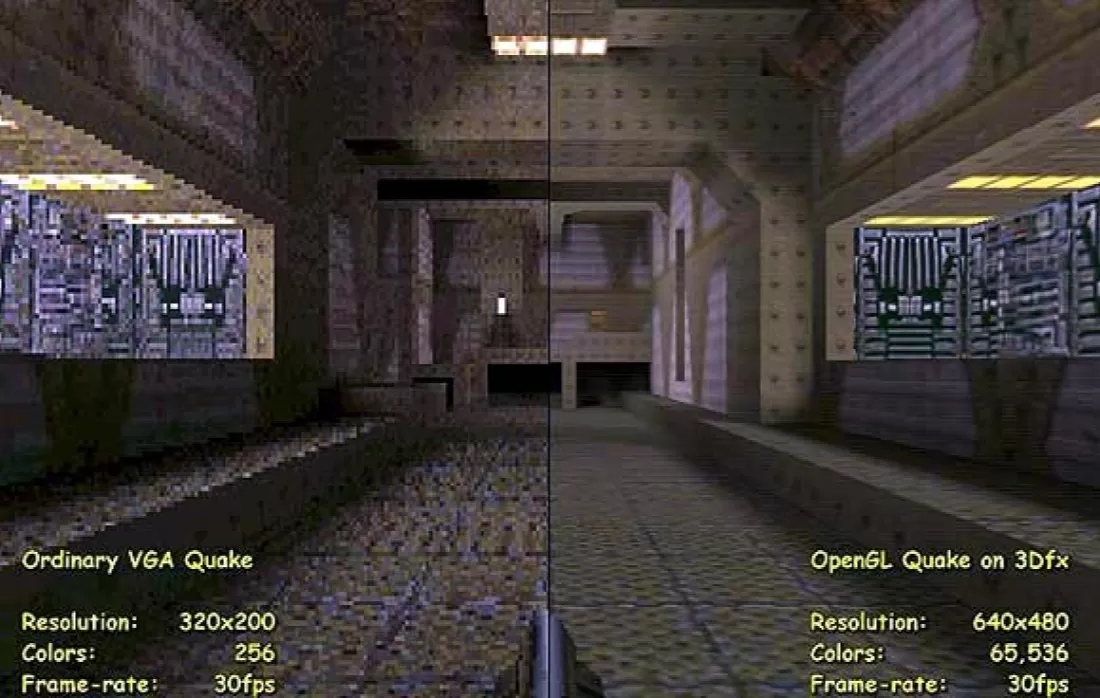
\includegraphics[width=0.8\linewidth]{fig/quake_3fx.png}
    \end{figure}
  \end{columns}
\end{frame}

%****************************************************************
% gpu-ri buruzko historio motz bat
%****************************************************************
\begin{frame}{Une brève histoire des GPUs}{ATI contre NVIDIA}
  \begin{columns}[t]
    \column{7cm}
    \begin{itemize}[<+->]
      \item 1999 : Nvidia GeForce 256
        \begin{itemize}
         \item Premier GPU
         \item technologie materielle {\em Transform and Lighting}\/ (T\&L)
         \item mémoire 32-64 Mo
         \item Fréquence GPU : 120 Mhz
         \item Fréquence Mémoire : 166-300Mhz
         \end{itemize}
      \item 2000 : ATI Radeon 7xxx
        \begin{itemize}
          \item techno T\&L
          \item mémoire 32-64Mo
          \item Fréquence GPU : 180-260Mhz
          \item Fréquence Mémoire : 360-460Mhz
          \item plusieurs cœurs de rendus
         \end{itemize}
    \end{itemize} 
    \column{5cm}
\begin{figure}[htbp]
  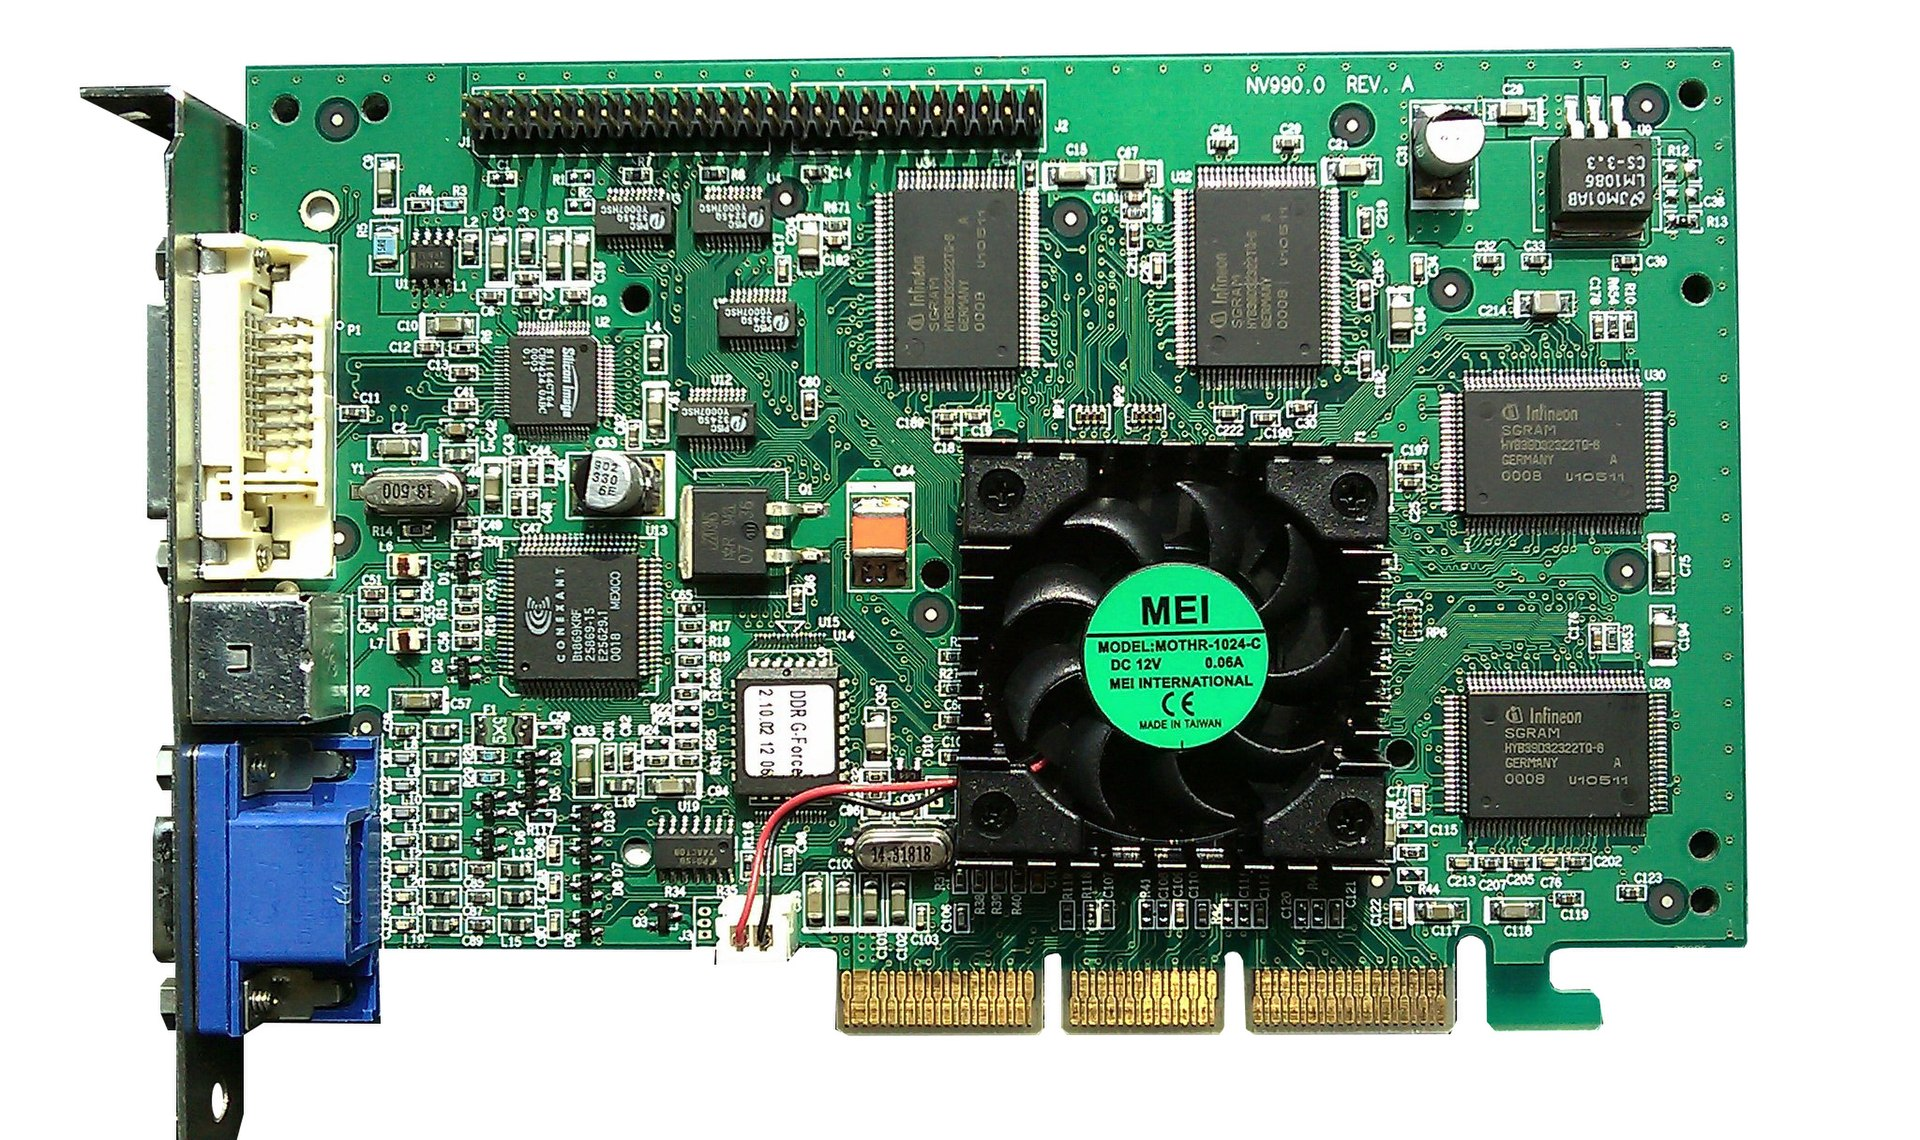
\includegraphics[width=0.7\linewidth]{fig/geforce256.jpg}
      \caption{\tiny Nvidia  GeForce 256}
 \end{figure}
\begin{figure}[htbp]
  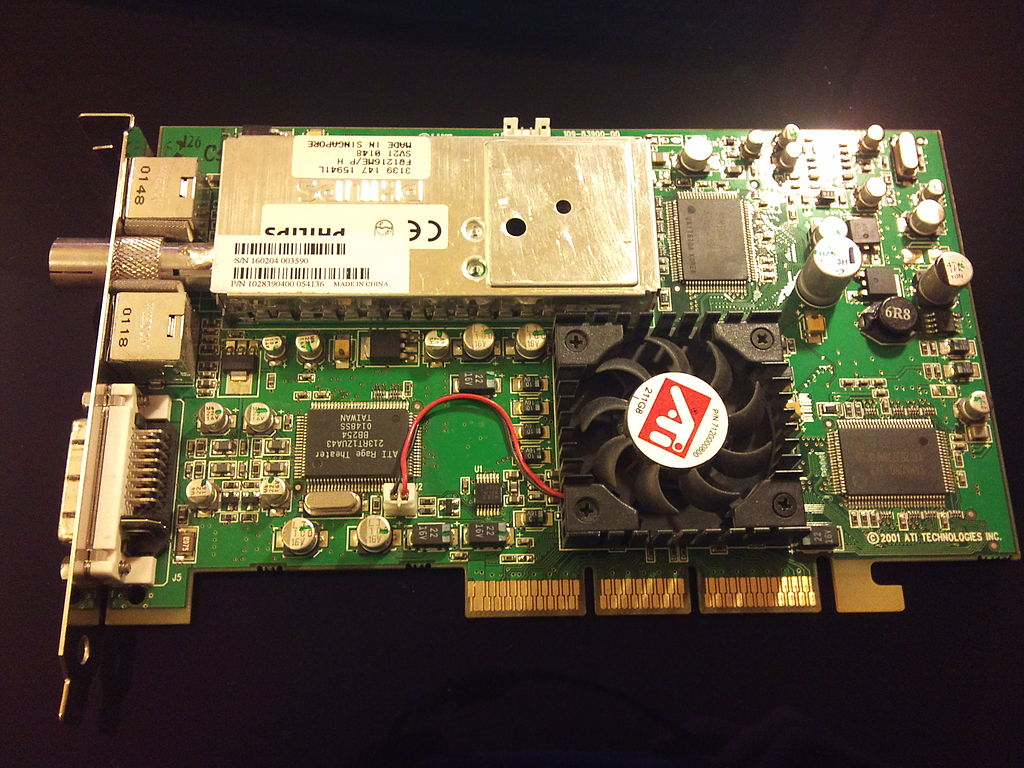
\includegraphics[width=0.8\linewidth]{fig/radeon7500.jpg}
      \caption{\tiny ATI Radeon 7500}
    \end{figure}
  \end{columns}
\end{frame}

%****************************************************************
% gpu-ri buruzko historio motz bat
%****************************************************************
\begin{frame}{Une brève histoire des GPUs}{l'ère des GPGPUs}
  \begin{columns}[t]
    \column{6cm}
    \begin{itemize}[<+->]
      \item 2001 : Nvidia GeForce 3 (NV20)
        \begin{itemize}
          \item unités programmables (nuanceurs)
         \end{itemize}
       \item les GPUs deviennent des accélérateurs de calcul génériques (GPGPU)
        \begin{itemize}
          \item les textures peuvent embarquer n'importe quelle donnée
          \item les {\em nuanceurs}\/ (shaders) peuvent pratiquement faire
            n'importe quel calcul
          \item OpenGL peut dorenavant être utiliser pour faire du calcul scientifique
         \end{itemize}
    \end{itemize} 
    \column{6cm}
\begin{figure}[htbp]
  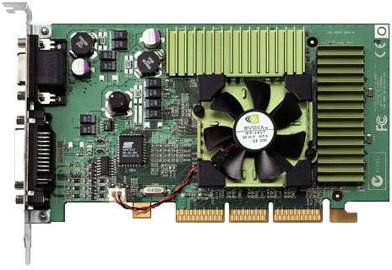
\includegraphics[width=0.8\linewidth]{fig/geforce3.jpg}
      \caption{\tiny Nvidia GeForce 3}
 \end{figure}
  \end{columns}
\end{frame}

%****************************************************************
% gpu-ri buruzko historio motz bat
%****************************************************************
\begin{frame}{Une brève histoire des GPUs}{les accélérateurs GPU}
  \begin{columns}[t]
    \column{6cm}
    \begin{itemize}[<+->]
      \item 2007 : Nvidia anticipe le marché possible et publie l'IPA CUDA
         Compute Unified Device Architecture)
      \item Nvidia lance aussi les accélérateurs Tesla
        \begin{itemize}
          \item sans sortie vidéo \harritu
          \item unités double précision
          \item code de correction d'erreurs (ECC mode) pour augmenter la robustesse
         \end{itemize}
       \item AMD (anciennement ATI) publie
        \begin{itemize}
          \item l'IPA «CLose to the Metal»
          \item le SDK «Stream»
        \end{itemize}
    \end{itemize} 
    \column{5cm}
\begin{figure}[htbp]
  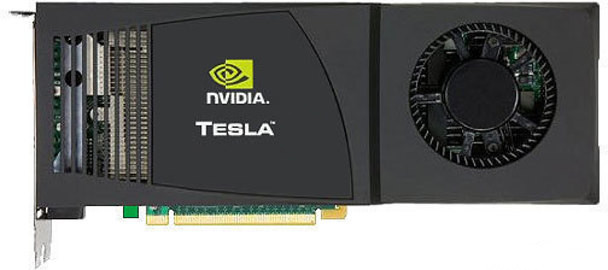
\includegraphics[width=0.7\linewidth]{fig/C1060.jpg}
      \caption{\tiny Tesla C1060}
 \end{figure}
\begin{figure}[htbp]
  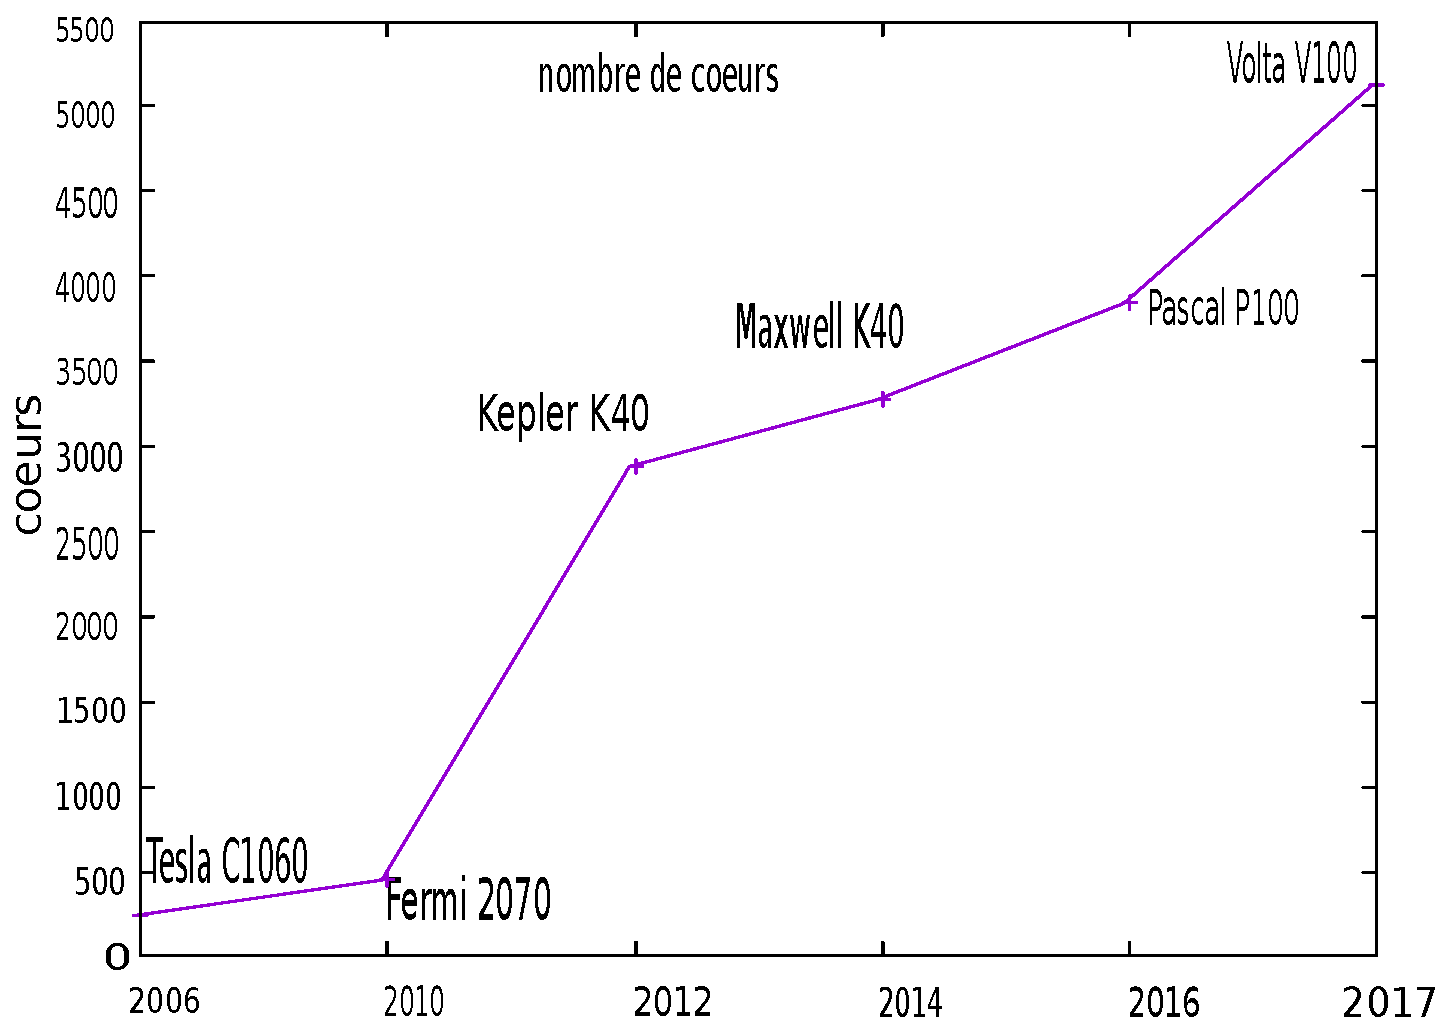
\includegraphics[height=4cm, width=0.9\linewidth]{fig/archis.eps}
 \end{figure}
  \end{columns}
\end{frame}

%****************************************************************
% gpu-ri buruzko historio motz bat
%****************************************************************
\begin{frame}{Une brève histoire des GPUs}{les dernières améliorations}
  \begin{columns}[t]
    \column{6cm}
    \begin{itemize}[<+->]
      \item Pascal :
        \begin{itemize}
          \item bus à haute-vitesse NVLink entre GPU et Hôte (jusqu'à 20Go/s)
          \item prise en charge de la demi-précision (16 bits)
          \item mémoire unifiée
         \end{itemize}
       \item Volta : 
        \begin{itemize}
          \item NVlink débit 25 Go/s
          \item cœurs Tenseurs : 
        \begin{itemize}
          \item opération FMA sur des matrices 4x4
          \item $D = A \times B + C$
          \item application aux réseaux de neurones
         \end{itemize}
        \end{itemize}
    \end{itemize} 
    \column{5cm}
\begin{figure}[htbp]
  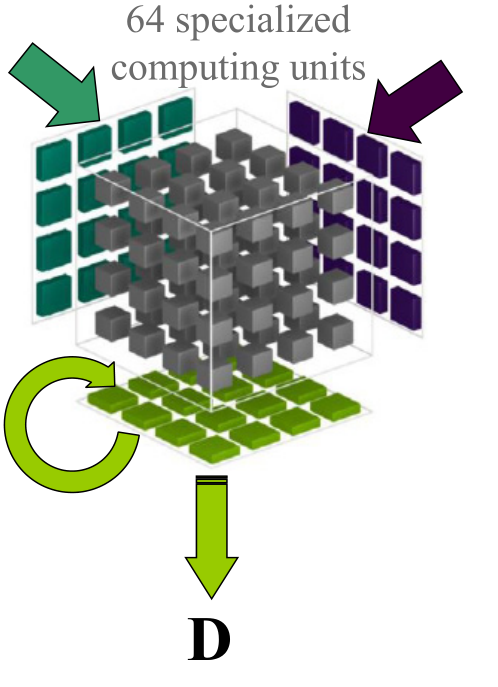
\includegraphics[width=0.7\linewidth]{fig/tensorCore.png}
 \end{figure}
\begin{figure}[htbp]
  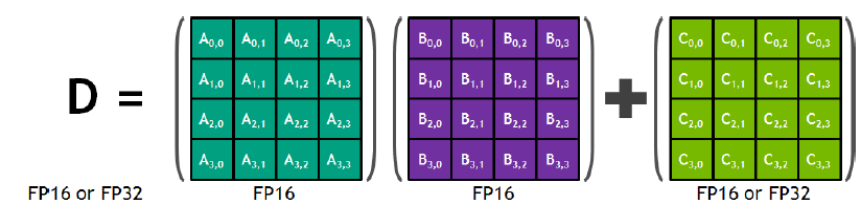
\includegraphics[width=0.9\linewidth]{fig/flux2.png}
 \end{figure}
  \end{columns}
\end{frame}

%****************************************************************
% liburutegiak
%****************************************************************
\begin{frame}{Interfaces de programmation applicatives}
  \begin{itemize}[<+->]
    \item langages (autre que C/C++) pour interfacer CUDA
  \begin{itemize}
    \item Fortran (compilateur PGI)
    \item Python, Julia et Matlab (avec cadriciels, Pytorch, flux.jl)
  \end{itemize} 
    \item bibliothèques optimisées pour CUDA
  \begin{itemize}
    \item Cublas et CuLA (algébre linéaire dense)
    \item Curand (génération de nombres aléatoires)
    \item CuFFT (transformées de fourier discrètes)
    \item CuDNN (apprentissage automatique)
    \item Cusparse (algèbre linéaire creuse)
    \item Thrust (CUDA à la mode STL)
    \item Magma (algébre linéaire sur archis hétérogènes)
  \end{itemize} 
    \item Standard OpenCL
  \begin{itemize}
    \item plus générique que CUDA 
    \item prise en charge des archi NVidia
    \item mais aussi d'AMD 
  \end{itemize} 
  \end{itemize} 
\end{frame}

%****************************************************************
% Apaimenak
%****************************************************************
\begin{frame}{Références}
\begin{itemize}[<+->]
  \item[\liburu] Cuda Fortran for Scientists and Engineers, G. Ruetsch, M. Fatica
  \item[\Pdf] Programming GPU Accelerators with OpenCL, R. Namyst, P.-A. Wacrenier \href{https://raymond-namyst.emi.u-bordeaux.fr/ens/pap/PAP-GPU.pdf}{\beamergotobutton{pdf}}
  \item[\Pdf] Performance Optimization Strategies For GPU-Accelerated Applications D. Goodwin \href{https://on-demand.gputechconf.com/gtc/2013/presentations/S3046-Performance-Optimization-Strategies-for-GPU-Accelerated-Apps.pdf}{\beamergotobutton{pdf}}
  \item[\faFilePowerpointO] CUDA Basics, S. Vialle \href{http://www.metz.supelec.fr/metz/personnel/vialle/course/PPS-5A-GPGPU/notes-de-cours-specifiques/PPS-GPU-02-CUDA-Basics-2spp.pdf}{\beamergotobutton{pdf}}
  \item[\Pdf] Understanding Latency Hiding on GPUs, V. Volkov \href{http://www2.eecs.berkeley.edu/Pubs/TechRpts/2016/EECS-2016-143.pdf}{\beamergotobutton{pdf}}
  \item[\Pdf] The Monte Carlo Method, N. Metropolis, S. Ulam,  Journal of the American Statistical Association Volume 44, 1949 
    \href{http://www.tandfonline.com/doi/abs/10.1080/01621459.1949.10483310}{\beamergotobutton{pdf}}
\end{itemize}
\end{frame}
\end{document}
